\begin{frame}
	\myheading{Module 11.5 : Image Classification continued (GoogLeNet and ResNet)}
\end{frame}

%%%%%%%%%%%%%%%%%%%%%%%%%%%%%%%%%%%%%%%%%%%%%%%%%%%%%%%%%%%%%%%%%%%%%%%%%%%%%%

\begin{frame}
	\begin{columns}
		\column{0.5\textwidth}
		\begin{overlayarea}{\textwidth}{\textheight}
			
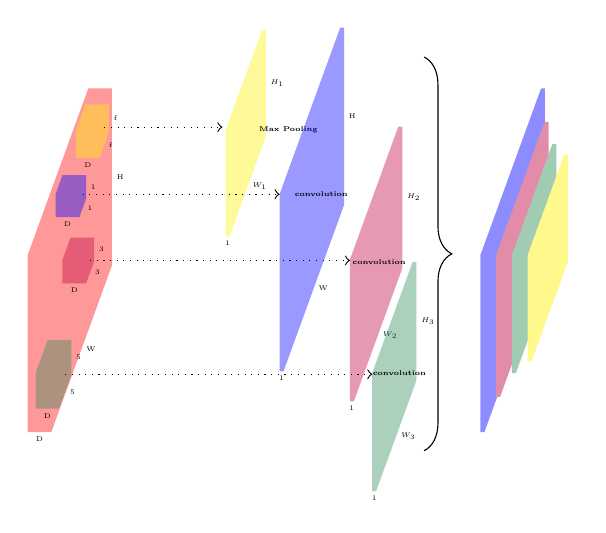
\begin{tikzpicture}[scale=0.5,transform shape]
	
	\pgfsetxvec{\pgfpoint{1cm}{0cm}}
	\pgfsetyvec{\pgfpoint{0cm}{1cm}}
	\pgfsetzvec{\pgfpoint{-.342cm}{-.94cm}}
	
	\def\cuboid#1#2#3#4#5{
	\begin{scope}
	\edef\mycolor{#2}
	\edef\depth{#3}
	\edef\height{#4}
	\edef\width{#5}
	\draw[black,fill=\mycolor, fill opacity=0.4, text opacity=1] #1 -- ++(-\depth,0,0) -- ++(0,-\height,0) -- ++(\depth,0,0) -- cycle #1 -- ++(0,0,-\width) -- ++(0,-\height,0) -- ++(0,0,\width) -- cycle  #1 -- ++(-\depth,0,0) -- ++(0,0,-\width) -- ++(\depth,0,0) -- cycle;
	\end{scope}
	}
	
	\def\cuboidlabel#1#2#3#4#5#6#7#8{
	\begin{scope}
	\edef\mycolor{#2}
	\edef\depth{#3}
	\edef\height{#4}
	\edef\width{#5}
	\edef\depthlabel{#6}
	\edef\heightlabel{#7}
	\edef\widthlabel{#8}
	\draw[draw=none,fill=\mycolor, fill opacity=0.4, text opacity=1] #1 -- ++(-\depth,0,0) -- ++(0,-\height,0) -- ++(\depth,0,0) node[pos=0.5,below] {\tiny \depthlabel} -- cycle #1 -- ++(0,0,-\width) -- ++(0,-\height,0) node[pos=0.5,right] {\tiny \heightlabel} -- ++(0,0,\width)  node[pos=0.5,below,right] {\tiny \widthlabel} -- cycle  #1 -- ++(-\depth,0,0) -- ++(0,0,-\width) -- ++(\depth,0,0) -- cycle;
	\end{scope}
	}
	
	\def\kernel#1#2#3#4#5#6{
	\begin{scope}
	\edef\mycolor{#2}
	\edef\depth{#3}
	\edef\height{#4}
	\edef\width{#5}
	\draw[black,fill=\mycolor, fill opacity=0.4, text opacity=1] #1 -- ++(-\depth,0,0) -- ++(0,-\height,0) -- ++(\depth,0,0) -- cycle #1 -- ++(0,0,-\width) -- ++(0,-\height,0) -- ++(0,0,\width) -- cycle  #1 -- ++(-\depth,0,0) -- ++(0,0,-\width) -- ++(\depth,0,0) -- cycle;
	
	\draw[dotted] #1 -- #6 #1++(0,0,-\width) -- #6 #1++(0,-\height,0) -- #6 #1++(0,-\height,-\width) -- #6;
	
	\end{scope}
	}
	
	\def\kernellabel#1#2#3#4#5#6#7#8#9{
	%#6 is target pixel
	\begin{scope}
	\edef\mycolor{#2}
	\edef\depth{#3}
	\edef\height{#4}
	\edef\width{#5}
	\edef\depthlabel{#7}
	\edef\heightlabel{#8}
	\edef\widthlabel{#9}
	\draw[draw=none,fill=\mycolor, fill opacity=0.4, text opacity=1] #1 -- ++(-\depth,0,0) -- ++(0,-\height,0) -- ++(\depth,0,0) node[pos=0.5,below] {\tiny \depthlabel} -- cycle #1 -- ++(0,0,-\width) -- ++(0,-\height,0) node[pos=0.5,right] {\tiny \heightlabel} -- ++(0,0,\width)  node[pos=0.5,below,right] {\tiny \widthlabel} -- cycle  #1 -- ++(-\depth,0,0) -- ++(0,0,-\width) -- ++(\depth,0,0) -- cycle;
	\end{scope}
	}
	
	\def\kernellabell#1#2#3#4#5#6#7#8#9{
	%#6 is target pixel
	\begin{scope}
	\edef\mycolor{#2}
	\edef\depth{#3}
	\edef\height{#4}
	\edef\width{#5}
	\edef\depthlabel{#7}
	\edef\heightlabel{#8}
	\edef\widthlabel{#9}
	\draw[draw=none,fill=\mycolor,  text opacity=1] #1 -- ++(-\depth,0,0) -- ++(0,-\height,0) -- ++(\depth,0,0) node[pos=0.5,below] {} -- cycle #1 -- ++(0,0,-\width) -- ++(0,-\height,0) node[pos=0.5,right] {} -- ++(0,0,\width)  node[pos=0.5,below,right] {} -- cycle  #1 -- ++(-\depth,0,0) -- ++(0,0,-\width) -- ++(\depth,0,0) -- cycle;
	
	%\draw[->] #10 -- #6 ;%#1++(0,0,-\width) -- #6 #1++(0,-\height,0) -- #6 #1++(0,-\height,-\width) -- #6;
	\end{scope}
	}
	
	
	%alexnet
	\onslide<1->{
	\cuboidlabel{(2,-0.5,-0.5)}{red}{0.6}{4.5}{4.5}{D}{H}{W}
	}
	
	\onslide<2->{
	\kernellabel{(2.2,-0.15,-3.5)}{yellow}{0.6}{0.7}{0.7}{(3.7,-2.5,-2.5)}{D}{f}{f}
	\draw [dotted,->] (2.2, -0.4,-3.85) -- (5.2, -0.4, -3.85);
	\kernellabel{(5.5,-0.15,-3.5)}{yellow}{0.1}{2.7}{2.7}{(3.7,-2.5,-2.5)}{1}{$H_1$}{$W_1$}
	\node (T) at (7,-0.15,-3.5){\textbf{\tiny{Max Pooling}}};
	
	}
	
	\onslide<3->{
	\kernellabel{(2.2,-0.35,-2)}{blue}{0.6}{0.6}{0.5}{(3.7,-2.5,-2.5)}{D}{1}{1}
	\draw [dotted,->] (2.2, -0.6,-2.25) -- (7.2, -0.6, -2.25);
	\kernellabel{(7.3,-0.6,-2.25)}{blue}{0.1}{4.5}{4.5}{(3.7,-2.5,-2.5)}{1}{H}{W}
	\node (T) at (8.3,-0.35,-2){\textbf{\tiny{\text{ convolution}}}};
	}
	
	\onslide<4->{
	\kernellabel{(2.2,-2.5,-2.5)}{purple}{0.6}{0.6}{0.6}{(3.7,-2.5,-2.5)}{D}{3}{3}
	\draw [dotted,->] (2.2,-2.8,-2.8) -- (8.8,-2.8,-2.8);
	\kernellabel{(9,-2.5,-2.5)}{purple}{0.1}{3.6}{3.6}{(3.7,-2.5,-2.5)}{1}{$H_2$}{$W_2$}
	\node (T) at (9.6,-2.55,-2.5){\textbf{\tiny{\text{ convolution}}}};
	}
	
	\onslide<5->{
	\kernellabel{(2.2,-3.5,-0.5)}{SeaGreen}{0.6}{0.9}{0.9}{(3.7,-2.5,-2.5)}{D}{5}{5}
	\draw [dotted,->] (2.2,-3.95,-0.95) -- (10,-3.95,-0.95);
	\kernellabel{(10.25,-3.5,-0.5)}{SeaGreen}{0.1}{3}{3}{(3.7,-2.5,-2.5)}{1}{$H_3$}{$W_3$}
	\node (T) at (10.8,-3.5,-0.5){\textbf{\tiny{\text{ convolution}}}};
	}
	
	
	\onslide<7->{
	\draw [decorate,decoration={brace,amplitude=10pt, mirror},xshift=4pt,yshift=0pt]
	(11.5,-5,0) -- (11.5, 5,0) node [black,midway,xshift=0.6cm] 
	{};
	}
	\onslide<7->{
	\kernellabell{(13,-0.5,-0.5)}{blue!45!white}{0.1}{4.5}{4.5}{(3.7,-2.5,-2.5)}{D}{5}{5}
	\kernellabell{(13.4,-0.5,-0.5)}{purple!45!white}{0.1}{3.6}{3.6}{(3.7,-2.5,-2.5)}{D}{5}{5}
	\kernellabell{(13.8,-0.5,-0.5)}{SeaGreen!45!white}{0.1}{3}{3}{(3.7,-2.5,-2.5)}{D}{5}{5}
	\kernellabell{(14.2,-0.5,-0.5)}{yellow!45!white}{0.1}{2.7}{2.7}{(3.7,-2.5,-2.5)}{1}{5}{5}

}
\end{tikzpicture}

		\end{overlayarea}
		\column{0.5\textwidth}
		\begin{overlayarea}{\textwidth}{\textheight}
			\onslide<1->{
				\begin{itemize}
					\justifying
					\item<1-> Consider the output at a certain layer of a convolutional neural network
					\item<2-> After this layer we could apply a maxpooling layer 
					\item<3-> Or a $1\times1$ convolution
					\item<4-> Or a $3\times3$ convolution
					\item<5-> Or a $5\times5$ convolution
					\item<6-> \textbf{Question:} Why choose between these options (convolution, maxpooling, filter sizes)?
					\item<7-> \textbf{Idea:} Why not apply all of them at the same time and then concatenate the feature maps?
					
				\end{itemize}
			}
		\end{overlayarea}
	\end{columns}
\end{frame}

%%%%%%%%%%%%%%%%%%%%%%%%%%%%%%%%%%%%%%%%%%%%%%%%%%%%%%%%%%%%%%%%%%%%%%%%%%%%%%

\begin{frame}
	\begin{columns}
		\column{0.5\textwidth}
		\begin{overlayarea}{\textwidth}{\textheight}
			
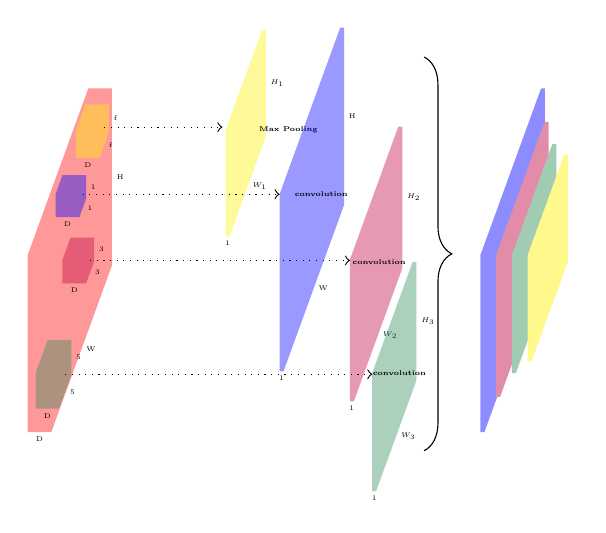
\begin{tikzpicture}[scale=0.5,transform shape]

\pgfsetxvec{\pgfpoint{1cm}{0cm}}
\pgfsetyvec{\pgfpoint{0cm}{1cm}}
\pgfsetzvec{\pgfpoint{-.342cm}{-.94cm}}

\def\cuboid#1#2#3#4#5{
\begin{scope}
\edef\mycolor{#2}
\edef\depth{#3}
\edef\height{#4}
\edef\width{#5}
\draw[black,fill=\mycolor, fill opacity=0.4, text opacity=1] #1 -- ++(-\depth,0,0) -- ++(0,-\height,0) -- ++(\depth,0,0) -- cycle #1 -- ++(0,0,-\width) -- ++(0,-\height,0) -- ++(0,0,\width) -- cycle  #1 -- ++(-\depth,0,0) -- ++(0,0,-\width) -- ++(\depth,0,0) -- cycle;
\end{scope}
}

\def\cuboidlabel#1#2#3#4#5#6#7#8{
\begin{scope}
\edef\mycolor{#2}
\edef\depth{#3}
\edef\height{#4}
\edef\width{#5}
\edef\depthlabel{#6}
\edef\heightlabel{#7}
\edef\widthlabel{#8}
\draw[draw=none,fill=\mycolor, fill opacity=0.4, text opacity=1] #1 -- ++(-\depth,0,0) -- ++(0,-\height,0) -- ++(\depth,0,0) node[pos=0.5,below] {\tiny \depthlabel} -- cycle #1 -- ++(0,0,-\width) -- ++(0,-\height,0) node[pos=0.5,right] {\tiny \heightlabel} -- ++(0,0,\width)  node[pos=0.5,below,right] {\tiny \widthlabel} -- cycle  #1 -- ++(-\depth,0,0) -- ++(0,0,-\width) -- ++(\depth,0,0) -- cycle;
\end{scope}
}

\def\kernel#1#2#3#4#5#6{
\begin{scope}
\edef\mycolor{#2}
\edef\depth{#3}
\edef\height{#4}
\edef\width{#5}
\draw[black,fill=\mycolor, fill opacity=0.4, text opacity=1] #1 -- ++(-\depth,0,0) -- ++(0,-\height,0) -- ++(\depth,0,0) -- cycle #1 -- ++(0,0,-\width) -- ++(0,-\height,0) -- ++(0,0,\width) -- cycle  #1 -- ++(-\depth,0,0) -- ++(0,0,-\width) -- ++(\depth,0,0) -- cycle;

\draw[dotted] #1 -- #6 #1++(0,0,-\width) -- #6 #1++(0,-\height,0) -- #6 #1++(0,-\height,-\width) -- #6;

\end{scope}
}

\def\kernellabel#1#2#3#4#5#6#7#8#9{
%#6 is target pixel
\begin{scope}
\edef\mycolor{#2}
\edef\depth{#3}
\edef\height{#4}
\edef\width{#5}
\edef\depthlabel{#7}
\edef\heightlabel{#8}
\edef\widthlabel{#9}
\draw[draw=none,fill=\mycolor, fill opacity=0.4, text opacity=1] #1 -- ++(-\depth,0,0) -- ++(0,-\height,0) -- ++(\depth,0,0) node[pos=0.5,below] {\tiny \depthlabel} -- cycle #1 -- ++(0,0,-\width) -- ++(0,-\height,0) node[pos=0.5,right] {\tiny \heightlabel} -- ++(0,0,\width)  node[pos=0.5,below,right] {\tiny \widthlabel} -- cycle  #1 -- ++(-\depth,0,0) -- ++(0,0,-\width) -- ++(\depth,0,0) -- cycle;
\end{scope}
}

\def\kernellabell#1#2#3#4#5#6#7#8#9{
%#6 is target pixel
\begin{scope}
\edef\mycolor{#2}
\edef\depth{#3}
\edef\height{#4}
\edef\width{#5}
\edef\depthlabel{#7}
\edef\heightlabel{#8}
\edef\widthlabel{#9}
\draw[draw=none,fill=\mycolor,  text opacity=1] #1 -- ++(-\depth,0,0) -- ++(0,-\height,0) -- ++(\depth,0,0) node[pos=0.5,below] {} -- cycle #1 -- ++(0,0,-\width) -- ++(0,-\height,0) node[pos=0.5,right] {} -- ++(0,0,\width)  node[pos=0.5,below,right] {} -- cycle  #1 -- ++(-\depth,0,0) -- ++(0,0,-\width) -- ++(\depth,0,0) -- cycle;

%\draw[->] #10 -- #6 ;%#1++(0,0,-\width) -- #6 #1++(0,-\height,0) -- #6 #1++(0,-\height,-\width) -- #6;
\end{scope}
}


%alexnet
\onslide<1->{
\cuboidlabel{(2,-0.5,-0.5)}{red}{0.6}{4.5}{4.5}{D}{H}{W}
}

\onslide<1->{
\kernellabel{(2.2,-0.15,-3.5)}{yellow}{0.6}{0.7}{0.7}{(3.7,-2.5,-2.5)}{D}{f}{f}
\draw [dotted,->] (2.2, -0.4,-3.85) -- (5.2, -0.4, -3.85);
\kernellabel{(5.5,-0.15,-3.5)}{yellow}{0.1}{2.7}{2.7}{(3.7,-2.5,-2.5)}{1}{$H_1$}{$W_1$}
\node (T) at (7,-0.15,-3.5){\textbf{\tiny{Max Pooling}}};

}

\onslide<1->{
\kernellabel{(2.2,-0.35,-2)}{blue}{0.6}{0.6}{0.5}{(3.7,-2.5,-2.5)}{D}{1}{1}
\draw [dotted,->] (2.2, -0.6,-2.25) -- (7.2, -0.6, -2.25);
\kernellabel{(7.3,-0.6,-2.25)}{blue}{0.1}{4.5}{4.5}{(3.7,-2.5,-2.5)}{1}{H}{W}
\node (T) at (8.3,-0.35,-2){\textbf{\tiny{\text{ convolution}}}};
}

\onslide<1->{
\kernellabel{(2.2,-2.5,-2.5)}{purple}{0.6}{0.6}{0.6}{(3.7,-2.5,-2.5)}{D}{3}{3}
\draw [dotted,->] (2.2,-2.8,-2.8) -- (8.8,-2.8,-2.8);
\kernellabel{(9,-2.5,-2.5)}{purple}{0.1}{3.6}{3.6}{(3.7,-2.5,-2.5)}{1}{$H_2$}{$W_2$}
\node (T) at (9.6,-2.55,-2.5){\textbf{\tiny{\text{ convolution}}}};
}

\onslide<1->{
\kernellabel{(2.2,-3.5,-0.5)}{SeaGreen}{0.6}{0.9}{0.9}{(3.7,-2.5,-2.5)}{D}{5}{5}
\draw [dotted,->] (2.2,-3.95,-0.95) -- (10,-3.95,-0.95);
\kernellabel{(10.25,-3.5,-0.5)}{SeaGreen}{0.1}{3}{3}{(3.7,-2.5,-2.5)}{1}{$H_3$}{$W_3$}
\node (T) at (10.8,-3.5,-0.5){\textbf{\tiny{\text{ convolution}}}};
}


\onslide<1->{
\draw [decorate,decoration={brace,amplitude=10pt, mirror},xshift=4pt,yshift=0pt]
(11.5,-5,0) -- (11.5, 5,0) node [black,midway,xshift=0.6cm] 
{};
}
\onslide<1->{
\kernellabell{(13,-0.5,-0.5)}{blue!45!white}{0.1}{4.5}{4.5}{(3.7,-2.5,-2.5)}{D}{5}{5}
\kernellabell{(13.4,-0.5,-0.5)}{purple!45!white}{0.1}{3.6}{3.6}{(3.7,-2.5,-2.5)}{D}{5}{5}
\kernellabell{(13.8,-0.5,-0.5)}{SeaGreen!45!white}{0.1}{3}{3}{(3.7,-2.5,-2.5)}{D}{5}{5}
\kernellabell{(14.2,-0.5,-0.5)}{yellow!45!white}{0.1}{2.7}{2.7}{(3.7,-2.5,-2.5)}{1}{5}{5}






}
\end{tikzpicture}

		\end{overlayarea}
		\column{0.5\textwidth}
		\begin{overlayarea}{\textwidth}{\textheight}
			\begin{itemize}
				\justifying
				\item<1-> Well this naive idea could result in a large number of computations
				\item<2-> If $P=0$ \& $S=1$ then convolving a $W \times H \times D$ input with a 
				$F \times F \times D$ filter results in a $(W - F + 1)(H - F + 1)$ sized output
				\item<3-> Each element of the output requires $O(F \times F \times D)$ computations
				\item<4-> Can we reduce the number of computations?
			\end{itemize}
		\end{overlayarea}
	\end{columns}
\end{frame}

%%%%%%%%%%%%%%%%%%%%%%%%%%%%%%%%%%%%%%%%%%%%%%%%%%%%%%%%%%%%%%%%%%%%%%%%%%%%%%

\begin{frame}
	\begin{columns}
		\column{0.5\textwidth}
		\begin{overlayarea}{\textwidth}{\textheight}
			\begin{center}
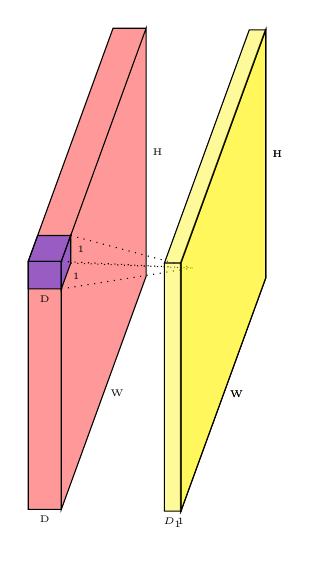
\begin{tikzpicture}[scale=0.7,transform shape]

\pgfsetxvec{\pgfpoint{1cm}{0cm}}
\pgfsetyvec{\pgfpoint{0cm}{1cm}}
\pgfsetzvec{\pgfpoint{-.342cm}{-.94cm}}

\def\cuboid#1#2#3#4#5{
\begin{scope}
\edef\mycolor{#2}
\edef\depth{#3}
\edef\height{#4}
\edef\width{#5}
\draw[black,fill=\mycolor, fill opacity=0.4, text opacity=1] #1 -- ++(-\depth,0,0) -- ++(0,-\height,0) -- ++(\depth,0,0) -- cycle #1 -- ++(0,0,-\width) -- ++(0,-\height,0) -- ++(0,0,\width) -- cycle  #1 -- ++(-\depth,0,0) -- ++(0,0,-\width) -- ++(\depth,0,0) -- cycle;
\end{scope}
}

\def\cuboidlabel#1#2#3#4#5#6#7#8{
\begin{scope}
\edef\mycolor{#2}
\edef\depth{#3}
\edef\height{#4}
\edef\width{#5}
\edef\depthlabel{#6}
\edef\heightlabel{#7}
\edef\widthlabel{#8}
\draw[draw=black,fill=\mycolor, fill opacity=0.4, text opacity=1] #1 -- ++(-\depth,0,0) -- ++(0,-\height,0) -- ++(\depth,0,0) node[pos=0.5,below] {\tiny \depthlabel} -- cycle #1 -- ++(0,0,-\width) -- ++(0,-\height,0) node[pos=0.5,right] {\tiny \heightlabel} -- ++(0,0,\width)  node[pos=0.5,below,right] {\tiny \widthlabel} -- cycle  #1 -- ++(-\depth,0,0) -- ++(0,0,-\width) -- ++(\depth,0,0) -- cycle;
\end{scope}
}

\def\kernel#1#2#3#4#5#6{
\begin{scope}
\edef\mycolor{#2}
\edef\depth{#3}
\edef\height{#4}
\edef\width{#5}
\draw[black,fill=\mycolor, fill opacity=0.4, text opacity=1] #1 -- ++(-\depth,0,0) -- ++(0,-\height,0) -- ++(\depth,0,0) -- cycle #1 -- ++(0,0,-\width) -- ++(0,-\height,0) -- ++(0,0,\width) -- cycle  #1 -- ++(-\depth,0,0) -- ++(0,0,-\width) -- ++(\depth,0,0) -- cycle;

\draw[dotted] #1 -- #6 #1++(0,0,-\width) -- #6 #1++(0,-\height,0) -- #6 #1++(0,-\height,-\width) -- #6;

\end{scope}
}

\def\kernellabel#1#2#3#4#5#6#7#8#9{
%#6 is target pixel
\begin{scope}
\edef\mycolor{#2}
\edef\depth{#3}
\edef\height{#4}
\edef\width{#5}
\edef\depthlabel{#7}
\edef\heightlabel{#8}
\edef\widthlabel{#9}
\draw[draw=black,fill=\mycolor, fill opacity=0.4, text opacity=1] #1 -- ++(-\depth,0,0) -- ++(0,-\height,0) -- ++(\depth,0,0) node[pos=0.5,below] {\tiny \depthlabel} -- cycle #1 -- ++(0,0,-\width) -- ++(0,-\height,0) node[pos=0.5,right] {\tiny \heightlabel} -- ++(0,0,\width)  node[pos=0.5,below,right] {\tiny \widthlabel} -- cycle  #1 -- ++(-\depth,0,0) -- ++(0,0,-\width) -- ++(\depth,0,0) -- cycle;

\draw[dotted] #1 -- #6 #1++(0,0,-\width) -- #6 #1++(0,-\height,0) -- #6 #1++(0,-\height,-\width) -- #6;

\end{scope}
}

%alexnet
\onslide<2->{
\cuboidlabel{(2,-0.5,-0.5)}{red}{0.6}{4.5}{4.5}{D}{H}{W}
}
\onslide<3->{
\kernellabel{(2,-0.5,-0.5)}{blue}{0.6}{0.5}{0.5}{(3.7,-2.5,-2.5)}{D}{1}{1}
}
\onslide<3>{
\cuboidlabel{(4,-1,-1)}{yellow}{0.01}{4.5}{4.5}{1}{H}{W}
}

%\onslide<6->{
%\kernellabel{(2,-1.5,-1.5)}{blue}{0.3}{0.5}{0.5}{(3.7,-2.5,-2.5)}{$D_1$}{1}{1}
%}
\onslide<4->{
\cuboidlabel{(4,-1,-1)}{yellow}{0.3}{4.5}{4.5}{$D_1$}{H}{W}
}
\end{tikzpicture}
\end{center}


		\end{overlayarea}
		\column{0.5\textwidth}
		\begin{overlayarea}{\textwidth}{\textheight}
			\begin{itemize}
				\justifying
				\item<1-> Yes, by using $1 \times 1$ convolutions
				\item<2-> Huh?? What does a $1 \times 1$ convolution do ?
				\item<3-> It aggregates along the depth
				\item<4-> So convolving a $D \times W \times H$ input with $D_1$ $1 \times 1\ (D_1 < D)$ filters will result
				in a $D_1 \times W \times H$ output ($S=1, P=0$)
				\item<5-> If $D_1<D$ then this effectively reduces the dimension of the input and hence the computations
				\item<6-> Specifically instead of O($F\times F\times D$) we will need O($F\times F\times D_1$) computations
				\item<7-> We could then apply subsequent $3\times 3$, $5\times 5$ filter on this reduced output  
			\end{itemize}
		\end{overlayarea}
	\end{columns}
\end{frame}

%%%%%%%%%%%%%%%%%%%%%%%%%%%%%%%%%%%%%%%%%%%%%%%%%%%%%%%%%%%%%%%%%%%%%%%%%%%%%%

\begin{frame}
	\begin{columns}
		\column{0.5\textwidth}
		\begin{overlayarea}{\textwidth}{\textheight}
			
	\begin{tikzpicture}[scale=0.4,transform shape]
		
		\pgfsetxvec{\pgfpoint{1cm}{0cm}}
		\pgfsetyvec{\pgfpoint{0cm}{1cm}}
		\pgfsetzvec{\pgfpoint{-.5cm}{-.866cm}}
		
		\def\cuboid#1#2#3#4#5#6{
			\begin{scope}
			\edef\mycolor{#2}
			\edef\depth{#3}
			\edef\height{#4}
			\edef\width{#5}
			\edef\op{#6}
			\draw[black,fill=\mycolor, fill opacity=\op] #1 -- ++(-\depth,0,0) -- ++(0,-\height,0) -- ++(\depth,0,0) -- cycle #1 -- ++(0,0,-\width) -- ++(0,-\height,0) -- ++(0,0,\width) -- cycle  #1 -- ++(-\depth,0,0) -- ++(0,0,-\width) -- ++(\depth,0,0) -- cycle;
			\end{scope}
		}
		
		\def\cuboidlabel#1#2#3#4#5#6#7#8{
			\begin{scope}
			\edef\mycolor{#2}
			\edef\depth{#3}
			\edef\height{#4}
			\edef\width{#5}
			\edef\depthlabel{#6}
			\edef\heightlabel{#7}
			\edef\widthlabel{#8}
			\draw[draw=black,fill=red, fill opacity=0.4] #1 -- ++(-\depth,0,0) -- ++(0,-\height,0) -- ++(\depth,0,0) node[pos=0.5,below] {\small \depthlabel} -- cycle #1 -- ++(0,0,-\width) -- ++(0,-\height,0) node[pos=0.5,right] {\small \heightlabel} -- ++(0,0,\width)  node[pos=0.5,below,right] {\small \widthlabel} -- cycle  #1 -- ++(-\depth,0,0) -- ++(0,0,-\width) -- ++(\depth,0,0) -- cycle;
			\end{scope}
		}
		
		\def\kernel#1#2#3#4#5#6{
			\begin{scope}
			\edef\mycolor{#2}
			\edef\depth{#3}
			\edef\height{#4}
			\edef\width{#5}
			\draw[black,fill=\mycolor, fill opacity=1] #1 -- ++(-\depth,0,0) -- ++(0,-\height,0) -- ++(\depth,0,0) -- cycle #1 -- ++(0,0,-\width) -- ++(0,-\height,0) -- ++(0,0,\width) -- cycle  #1 -- ++(-\depth,0,0) -- ++(0,0,-\width) -- ++(\depth,0,0) -- cycle;
			
			\draw[dotted] #1 -- #6 #1++(0,0,-\width) -- #6 #1++(0,-\height,0) -- #6 #1++(0,-\height,-\width) -- #6;
			
			\end{scope}
		}
		
		\def\kernellabel#1#2#3#4#5#6#7#8#9{
			%#6 is target pixel
			\begin{scope}
			\edef\mycolor{#2}
			\edef\depth{#3}
			\edef\height{#4}
			\edef\width{#5}
			\edef\depthlabel{#7}
			\edef\heightlabel{#8}
			\edef\widthlabel{#9}
			\draw[draw=black,fill=\mycolor, fill opacity=1] #1 -- ++(-\depth,0,0) -- ++(0,-\height,0) -- ++(\depth,0,0) node[pos=0.5,below] {\tiny \depthlabel} -- cycle #1 -- ++(0,0,-\width) -- ++(0,-\height,0) node[pos=0.5,right] {\tiny \heightlabel} -- ++(0,0,\width)  node[pos=0.5,below,right] {\tiny \widthlabel} -- cycle  #1 -- ++(-\depth,0,0) -- ++(0,0,-\width) -- ++(\depth,0,0) -- cycle;
			\end{scope}
		}
		
		\def\kernellabell#1#2#3#4#5#6#7#8#9{
			%#6 is target pixel
			\begin{scope}
			\edef\mycolor{#2}
			\edef\depth{#3}
			\edef\height{#4}
			\edef\width{#5}
			\edef\depthlabel{#7}
			\edef\heightlabel{#8}
			\edef\widthlabel{#9}
			\draw[draw=black,fill=\mycolor, fill opacity=1] #1 -- ++(-\depth,0,0) -- ++(0,-\height,0) -- ++(\depth,0,0) node[pos=0.5,below] {} -- cycle #1 -- ++(0,0,-\width) -- ++(0,-\height,0) node[pos=0.5,right] {} -- ++(0,0,\width)  node[pos=0.5,below,right] {} -- cycle  #1 -- ++(-\depth,0,0) -- ++(0,0,-\width) -- ++(\depth,0,0) -- cycle;
			\end{scope}
		}
		
		
		\onslide<1->{
				\pgfmathsetmacro{\seedx}{-3}
				\pgfmathsetmacro{\seedy}{1.5}
				 /

				\node [rectangle, text width=3cm, fill=purple!10, minimum height=4mm, minimum width=10mm] (C) at (2,2){\footnotesize $1 \times 1$ convolutions (dimensionality reduction)};
				\kernel{(-4.75,-1.5,-4)}{blue!50}{1.4}{0.5}{0.5}{(0.4,2,0)}


		}

		\onslide<1>{

				\node [rectangle, text width=3cm, fill=blue!50, minimum height=16mm, minimum width=10mm] (G) at (6,2){\footnotesize $3 \times 3$ convolutions (on reduced input)};
				\node [rectangle, text width=3cm, fill=blue!50, minimum height=16mm, minimum width=10mm] (H) at ($(G) + (0,-2)$){\footnotesize $5 \times 5$ convolutions (on reduced input)};
				\draw [->](C)--(G);
				\draw [->](C)--(H);

		}
		\onslide<2->{
				\node [rectangle, text width=3cm, fill=blue!50, minimum height=16mm, minimum width=10mm] (G) at (6,2){\footnotesize $3 \times 3$ convolutions (on reduced input)};
				\node [rectangle, text width=3cm, fill=blue!50, minimum height=16mm, minimum width=10mm] (H) at ($(G) + (0,-2)$){\footnotesize $5 \times 5$ convolutions (on reduced input)};
				\node [rectangle, text width=3cm, fill=purple!10, minimum height=4mm, minimum width=10mm] (D) at ($(C) + (0,-2)$){\footnotesize $1 \times 1$ convolutions (dimensionality reduction)};
				\draw[->](C)--(G);
				\draw[->](D)--(H);
				\kernel{(-4.5,-2.5,-3)}{blue!50}{1.4}{0.5}{0.5}{(0.4,0,0)}

		}
		\onslide<3->{
		\node [rectangle, text width=3cm,fill=yellow!50, minimum height=4mm, minimum width=10mm] (E) at ($(D) + (0,-2)$){\footnotesize $3 \times 3$ Maxpooling (dimensionality reduction)};
				\node [rectangle, text width=3cm, fill=purple!10, minimum height=16mm, minimum width=10mm, align=center] (I) at ($(H) + (0,-2)$){\footnotesize $1 \times 1$ convolutions};
				\kernel{(-3.5,-2.5,-1)}{yellow}{1.4}{0.8}{0.8}{(0.4,-2,0)}
					\draw[->](E)--(I);

		}

		\onslide<4->{
					\node [rectangle, text width=3cm, fill=purple!10, minimum height=4mm, minimum width=10mm] (D) at ($(C) + (0,-2)$){\footnotesize $1 \times 1$ convolutions (dimensionality reduction)};
				\kernel{(-4.5,-2.5,-3)}{blue!50}{1.4}{0.5}{0.5}{(0.4,0,0)}
		
				\kernel{(-3.75,0.2,-4.1)}{blue!50}{1.4}{0.5}{0.5}{(5,4,0)}
				\node [rectangle, text width=3cm, fill=blue!50, minimum height=16mm, minimum width=10mm, align=center] (B) at (6,4){\footnotesize  {$1 \times 1$ convolutions} };
				\node [rectangle, text width=3cm, fill=blue!50, minimum height=16mm, minimum width=10mm] (G) at ($(B) + (0,-2)$){\footnotesize $3 \times 3$ convolutions (on reduced input)};
				\node [rectangle, text width=3cm, fill=blue!50, minimum height=16mm, minimum width=10mm] (H) at ($(G) + (0,-2)$){\footnotesize $5 \times 5$ convolutions (on reduced input)};
				\node [rectangle, text width=3cm, fill=purple!10, minimum height=16mm, minimum width=10mm, align=center] (I) at ($(H) + (0,-2)$){\footnotesize $1 \times 1$ convolutions};
				\draw[->](C)--(G);
				\draw[->](D)--(H);

		}	
		\onslide<5->{
				\node [rectangle, text width=3cm, fill=green!20, minimum height=16mm, minimum width=10mm, align=center] (L) at (12,1){Filter\ \ \ \ \ \ \ \ \ \ \ \ \ \ concatenation};
				\draw [->](B)--(L);
				\draw [->](G)--(L);
				\draw [->](H)--(L);
				\draw [->](I)--(L);
		}

		\onslide<1->{

				\cuboidlabel{(0+\seedx,0+\seedy,0)}{red}{1.4}{4.5}{4.5}{256}{28}{28}

		}
		\end{tikzpicture}
		

		\end{overlayarea}
		\column{0.5\textwidth}
		\begin{overlayarea}{\textwidth}{\textheight}
			\begin{itemize}
				\justifying
				\item<1-> But we might want to use different dimensionality reductions before the $3 \times 3$ and $5 \times 5$ filters
				\item<2-> So we can use $D_1$ and $D_2$ $1\times 1$ filters before the $3 \times 3$ and $5 \times 5$ filters respectively
				\item<3-> We can then add the maxpooling layer followed by dimensionality reduction
				\item<4-> And a new set of $1\times 1$ convolutions
				\item<5-> And finally we concatenate all these layers
				\item<6-> This is called the \textbf{Inception module}
				\item<7-> We will now see \textbf{GoogLeNet} which contains many such inception modules
			\end{itemize}
		\end{overlayarea}
	\end{columns}
\end{frame}

%%%%%%%%%%%%%%%%%%%%%%%%%%%%%%%%%%%%%%%%%%%%%%%%%%%%%%%%%%%%%%%%%%%%%%%%%%%%%%

\begin{frame}
	\begin{center}
\hspace*{-1.1cm}
        \begin{tikzpicture}[scale=0.25]
       
    \onslide<1->{   \renewcommand{\forefillColor}{black!50!white}
        \renewcommand{\borderColor}{white}
        \renewcommand{\toprsidefillcolor}{red}
        %% input layer
        \handmadecube{0}{5.5}{3.5}{-1}{0}
        \renewcommand{\toprsidefillcolor}{green}
                                
        \handmadecube{0}{5.5}{3.5}{-1+0.2}{0}
\renewcommand{\toprsidefillcolor}{blue!60!white}
                        
        \handmadecube{0}{5.5}{3.5}{-1+0.4}{0}
        \node[scale=0.6] at (1-0.6*2.6-0.1,0-4.8-1){\tiny{Input}};
        \node [scale=0.5, rotate=53] at (1-0.6*2.6+0.6,0.2) {\tiny{229}};
        \node [scale=0.5, rotate=90] at (1-0.6*2.6+0.2,-2) {\tiny{229}};
        
       
        }
        %% convolution 
        \onslide<2->{  
             \renewcommand{\forefillColor}{red!50!white}
            \renewcommand{\borderColor}{white}
            \renewcommand{\toprsidefillcolor}{red!50!white!50}
        
                \pgfmathsetmacro{\seedx}{1+0.8}
                \pgfmathsetmacro{\seedy}{0}
                \pgfmathsetmacro{\anim}{1}
                \foreach \xct in {1,...,1}
               {
                    
                   \pgfmathparse{int(\anim+\xct)}
                    \onslide<\pgfmathresult->{
                       \pgfmathsetmacro{\xcti}{\seedx+\xct*0.5}
                    \pgfmathsetmacro{\ycti}{\seedy}
                    \handmadecube{0.5}{4.5}{2.5}{\xcti}{\ycti}
                   }
                
                
                
               }
                \onslide<2->{\node[scale=0.6] at (1+1,0-4.8){\tiny{Conv}};}
                \onslide<2->{\node [scale=0.5, rotate=53] at (1-0.6*2.6-1+3.2+1.2,0.2) {\tiny{112}};
                \node [scale=0.5, rotate=90] at (1-0.6*2.6+0.2-1+2.6+1.2,-2) {\tiny{112}};
                \node[scale=0.5] at (1+0.725+0.32,0-4.2){\tiny{64}};}
              }
              
              \onslide<3->{
              \renewcommand{\forefillColor}{blue!50!white}
                                  \renewcommand{\borderColor}{white}
                                  \renewcommand{\toprsidefillcolor}{blue!50!white!50}
                                  \pgfmathsetmacro{\seedx}{3.9}
                                  \pgfmathsetmacro{\seedy}{0}
                                                
                                  \foreach \xct/\yct in {1}
                                  {
                                      
                                      \pgfmathsetmacro{\xcti}{\seedx+\xct*0.5}
                                      \pgfmathsetmacro{\ycti}{\seedy}
                                      \handmadecube{0.5}{3.8}{1.8}{\xcti}{\ycti}
                                  }
                                  \node[scale=0.6] at (1+2.8,0-4.2){\tiny{maxpool}};
                                  \node [scale=0.5, rotate=53] at (1+3.7+0.2,0.2) {\tiny{56}};
                                  \node [scale=0.5, rotate=90] at (1+3.3+0.2,-2+0.5) {\tiny{56}};
                                  \node[scale=0.5] at (1+2.85+0.3,0-3.5){\tiny{64}};
                                  
              }
              
              \onslide<4->{
               \renewcommand{\forefillColor}{red!50!white}
                                 \renewcommand{\borderColor}{white}
                                 \renewcommand{\toprsidefillcolor}{red!50!white!50}
                                 \pgfmathsetmacro{\seedx}{5.5}
                                 \pgfmathsetmacro{\seedy}{0}
                                 \pgfmathsetmacro{\anim}{4}
                                 \foreach \xct in {1,...,1}
                                 {
                                     
                                     
                                     \pgfmathsetmacro{\xcti}{\seedx+\xct}
                                     \pgfmathsetmacro{\ycti}{\seedy}
                                     \handmadecube{0.95}{3.8}{1.8}{\xcti}{\ycti}
                                 }   
                             \node[scale=0.6] at (1+5.25-0.5,0-4.2){\tiny{Conv}};
                             \node [scale=0.5, rotate=53] at (1+6.7-0.6,0.2) {\tiny{56}};
                             \node [scale=0.5, rotate=90] at (1+6.4-0.6-0.1,-1.5) {\tiny{56}};
                             \node[scale=0.5] at (1+5.65-0.6,0-3.5){\tiny{192}};
              
              }
               \onslide<5->{       \renewcommand{\forefillColor}{blue!50!white}
                                      \renewcommand{\borderColor}{white}
                                      \renewcommand{\toprsidefillcolor}{blue!50!white!50}
                                      \pgfmathsetmacro{\shiftx}{1}
                                      \pgfmathsetmacro{\shifty}{0}
                                                                            
                                      \pgfmathsetmacro{\seedx}{8.1}
                                      \pgfmathsetmacro{\seedy}{0}
                                      
                                      \foreach \xct/\yct in {1}
                                      {
                                          \pgfmathsetmacro{\xcti}{\seedx+\xct*0.5}
                                          \pgfmathsetmacro{\ycti}{\seedy}
                                          \handmadecube{0.95}{3.3}{1.3    }{\xcti}{\ycti}
                                      }   
                                  
                                      \node[scale=0.6] at (1+7.8-0.7,0-3.6){\tiny{maxpool}};
                                      \node [scale=0.5, rotate=49] at (1+8.7-0.6,0.1) {\tiny{28}};
                                      \node [scale=0.5, rotate=90] at (1+8.5-0.7,-1.35) {\tiny{28}};
                                      \node[scale=0.5] at (1+7.8-0.7,0-3){\tiny{192}};
                                      
                                      }
                                      
                                      \onslide<6->{
                                      \renewcommand{\forefillColor}{orange!50!white}
                                                              \renewcommand{\borderColor}{white}
                                                              \renewcommand{\toprsidefillcolor}{orange!50!white!50}
                                                              \pgfmathsetmacro{\seedx}{10}
                                                              \pgfmathsetmacro{\seedy}{0}
                                                              \pgfmathsetmacro{\anim}{7}
                                                              \foreach \xct/\yct in {1,...,1}
                                                              {
                                                                  \pgfmathsetmacro{\xcti}{\seedx+1.35*\xct}
                                                                  \pgfmathsetmacro{\ycti}{\seedy}
                                                                  \handmadecube{1.9}{3.3}{1.3}{\xcti}{\ycti}
                                                              
                                                              }
                                                              
                                                                \node[scale=0.6] at (1+11.2-2+0.2,0-3.6){\tiny{Inception}};
                                                                 \node [scale=0.5, rotate=49] at (1+13.625-2.8,0.1) {\tiny{28}};
                                                                  \node [scale=0.5, rotate=90] at (1+13.425-2.8,-1.35) {\tiny{28}};
                                                                  \node[scale=0.5] at (1+12.6-3.2,0-3){\tiny{256}};
                                                                  \node[scale=0.5] at (1+12.6-3.2,0-3+1.5){\small{\textbf{3a}}};
                                                              
                                      }
                                      
                                      \onslide<7->{
															  \renewcommand{\forefillColor}{orange!50!white}
                                                              \renewcommand{\borderColor}{white}
                                                              \renewcommand{\toprsidefillcolor}{orange!50!white!50}
                                                              \pgfmathsetmacro{\seedx}{13.2}
                                                              \pgfmathsetmacro{\seedy}{0}
                                                              \pgfmathsetmacro{\anim}{7}
                                                              \foreach \xct/\yct in {1,...,1}
                                                              {
                                                                  \pgfmathsetmacro{\xcti}{\seedx+1.35*\xct}
                                                                  \pgfmathsetmacro{\ycti}{\seedy}
                                                                  \handmadecube{2.4}{3.3}{1.3}{\xcti}{\ycti}
                                                              
                                                              }
                                                              
                                                                \node[scale=0.6] at (1+11.2-2+0.2+2.9,0-3.6){\tiny{Inception}};
                                                                 \node [scale=0.5, rotate=49] at (1+13.625+0.3,0.1) {\tiny{28}};
                                                                  \node [scale=0.5, rotate=90] at (1+13.425+0.3,-1.35) {\tiny{28}};
                                                                  \node[scale=0.5] at (1+12.6-3.2+3,0-3){\tiny{480}};
                                                                  \node[scale=0.5] at (1+12.6-3.2+3,0-3+1.5){\small{\textbf{3b}}};
                                      }
                                      \onslide<8->{
                                      \renewcommand{\forefillColor}{blue!50!white}
                                      \renewcommand{\borderColor}{white}
                                      \renewcommand{\toprsidefillcolor}{blue!50!white!50}
                                      \pgfmathsetmacro{\seedx}{17.25}
                                      \pgfmathsetmacro{\seedy}{-0.2}
                                                                                      
                                      \foreach \xct/\yct in {1}
                                      {
                                                                            
                                      \pgfmathsetmacro{\xcti}{\seedx+\xct*0.5}
                                      \pgfmathsetmacro{\ycti}{\seedy}
                                      \handmadecube{2.4}{2.8}{1.2}{\xcti}{\ycti}
                                      }
                                      \node[scale=0.6] at (1+2.8+12.6,0-4.2+0.8){\tiny{maxpool}};
                                      \node [scale=0.5, rotate=53] at (1+3.7+0.2+13.5-0.4,0.2-0.4) {\tiny{14}};
                                      \node [scale=0.5, rotate=90] at (1+3.3+0.2+13.5,-2+0.5) {\tiny{14}};
                                      \node[scale=0.5] at (1+2.85+0.3+12.5,0-3.5+1-0.2){\tiny{480}};
                                                                        
                                                    }
                                                    
% %                                                    \onslide<9->{
                                      \renewcommand{\forefillColor}{orange!50!white}
                                                          \renewcommand{\borderColor}{white}
                                                              \renewcommand{\toprsidefillcolor}{orange!50!white!50}
                                                              \pgfmathsetmacro{\seedx}{21.3}
                                                              \pgfmathsetmacro{\seedy}{-0.2}
                                                              \pgfmathsetmacro{\anim}{9}
                                                              \foreach \xct/\yct in {0,...,2}
                                                              {
                                                                   \pgfmathparse{int(\anim+\xct)}
                                                                                              \onslide<\pgfmathresult->{
                                                                  \pgfmathsetmacro{\xcti}{\seedx+2.8*\xct}
                                                                  \pgfmathsetmacro{\ycti}{\seedy}
                                                                  \handmadecube{2.8}{2.8}{1.2}{\xcti}{\ycti}}
                                                              
                                                              }
                                                              
                                                               \onslide<9->{ \node[scale=0.6] at (1+11.2-2+0.2+12.5,0-4.2+0.8){\tiny{Inception}};
                                                               \node[scale=0.5] at (1+12.6-3.2+9.6,0-3+1.5){\small{\textbf{4a}}};
                                                               }
                                                                 \onslide<11->{\node [scale=0.5, rotate=49] at (1+13.625-2.8+15.5,0) {\tiny{14}};
                                                                  \node [scale=0.5, rotate=90] at (1+13.425-2.8+15.5,-2+0.5) {\tiny{14}};
                                                                  \node[scale=0.5] at (1+12.6-3.2+15,0-3.5+1-0.2){\tiny{512}};}
                                                                  % %4a

                                                                  % %4b
                                                                  \onslide<10->{\node[scale=0.5] at (1+12.6-3.2+10+2.5-0.2,0-3+1.5){\small{\textbf{4b}}};}
                                                                  % %4c
                                                                  \onslide<11->{\node[scale=0.5] at (1+12.6-3.2+10+5,0-3+1.5){\small{\textbf{4c}}};}
                                              % %     } % % % % % % % % % % % % %
                                              \onslide<12->{
 \renewcommand{\forefillColor}{orange!50!white}
                                                          \renewcommand{\borderColor}{white}
                                                              \renewcommand{\toprsidefillcolor}{orange!50!white!50}
                                                              \pgfmathsetmacro{\seedx}{30.6}
                                                              \pgfmathsetmacro{\seedy}{-0.2}
                                                              \pgfmathsetmacro{\anim}{12}
                                                              \foreach \xct/\yct in {0}
                                                              {
                                                                   \pgfmathparse{int(\anim+\xct)}
                                                                                              \onslide<\pgfmathresult->{
                                                                  \pgfmathsetmacro{\xcti}{\seedx+2.8*\xct}
                                                                  \pgfmathsetmacro{\ycti}{\seedy}
                                                                  \handmadecube{3}{2.8}{1.2}{\xcti}{\ycti}}
                                                              
                                                              }
                                                              
														\node[scale=0.6] at (1+11.2-2+0.2+18.6,0-4.2+0.8){\tiny{Inception}};
                                                               
\node [scale=0.5, rotate=49] at (1+13.625-2.8+17.6+1.5,0) {\tiny{14}};
                                                                  \node [scale=0.5, rotate=90] at (1+13.425-2.8+17.5+1.6,-2+0.5) {\tiny{14}};
                                                                  \node[scale=0.5] at (1+12.6-3.2+17+1.7,0-3.5+1-0.2){\tiny{528}};
                                                                  % %4a

                                                                  % %4b
                                                                  
                                                                  
                                                                  \node[scale=0.5] at (1+12.6-3.2+10+5+3+0.6,0-3+1.5){\small{\textbf{4d}}};
                                              }
\onslide<13->{
 \renewcommand{\forefillColor}{orange!50!white}
                                                          \renewcommand{\borderColor}{white}
                                                              \renewcommand{\toprsidefillcolor}{orange!50!white!50}
                                                              \pgfmathsetmacro{\seedx}{34.75}
                                                              \pgfmathsetmacro{\seedy}{-0.2}
                                                              \pgfmathsetmacro{\anim}{12}
                                                              \foreach \xct/\yct in {0}
                                                              {
                                                                   \pgfmathparse{int(\anim+\xct)}
                                                                   \onslide<\pgfmathresult->{
                                                                  \pgfmathsetmacro{\xcti}{\seedx+2.8*\xct}
                                                                  \pgfmathsetmacro{\ycti}{\seedy}
                                                                  \handmadecube{3.5}{2.8}{1.2}{\xcti}{\ycti}}
                                                              
                                                              }
                                                              
														\node[scale=0.6] at (1+11.2-2+0.2+18.5+4.3,0-4.2+0.8){\tiny{Inception}};
                                                               
\node [scale=0.5, rotate=49] at (1+13.625-2.8+17.6+1.5+4.3,0) {\tiny{14}};
\node [scale=0.5, rotate=90] at (1+13.425-2.8+17.5+1.6+4.3,-2+0.5) {\tiny{14}};
\node[scale=0.5] at (1+12.6-3.2+17+1.7+4,0-3.5+1-0.2){\tiny{832}};
                                                                  % %4a

                                                                  % %4b
                                                                  
                                                                  
                                                                  \node[scale=0.5] at (1+12.6-3.2+10+5+3+4.6,0-3+1.5){\small{\textbf{4e}}};
                                              }  
                                              
                                              \onslide<14->{

 \renewcommand{\forefillColor}{blue!50!white}
                                                          \renewcommand{\borderColor}{white}
                                                              \renewcommand{\toprsidefillcolor}{blue!50!white!50}
                                                              \pgfmathsetmacro{\seedx}{38.9}
                                                              \pgfmathsetmacro{\seedy}{-0.45}
                                                              \pgfmathsetmacro{\anim}{12}
                                                              \foreach \xct/\yct in {0}
                                                              {
                                                                   \pgfmathparse{int(\anim+\xct)}
                                                            blue       \onslide<\pgfmathresult->{
                                                                  \pgfmathsetmacro{\xcti}{\seedx+2.8*\xct}
                                                                  \pgfmathsetmacro{\ycti}{\seedy}
                                                                  \handmadecube{3.5}{2}{1}{\xcti}{\ycti}}
                                                              
                                                              }
                                                              
														\node[scale=0.6] at (1+11.2-2+0.2+18.5+4.3+4,0-4.2+0.8+0.4){\tiny{maxpool}};
                                                               
\node [scale=0.5, rotate=49] at (1+13.625-2.8+17.6+1.5+4.3+4,-0.4) {\tiny{7}};
\node [scale=0.5, rotate=90] at (1+13.425-2.8+17.5+1.6+4.3+4,-1.5) {\tiny{7}};
\node[scale=0.5] at (1+12.6-3.2+17+1.7+4+4,0-3.5+1+0.35){\tiny{832}};
                                                                  % %4a

                                                                  % %4b
                                                                  
   
                                              }
                                              
                                              \onslide<15->{
 \renewcommand{\forefillColor}{orange!50!white}
                                                          \renewcommand{\borderColor}{white}
                                                              \renewcommand{\toprsidefillcolor}{orange!50!white!50}
                                                              \pgfmathsetmacro{\seedx}{43}
                                                              \pgfmathsetmacro{\seedy}{-0.45}
                                                              \pgfmathsetmacro{\anim}{12}
                                                              \foreach \xct/\yct in {0}
                                                              {
                                                                   \pgfmathparse{int(\anim+\xct)}
                                                                   \onslide<\pgfmathresult->{
                                                                  \pgfmathsetmacro{\xcti}{\seedx+2.8*\xct}
                                                                  \pgfmathsetmacro{\ycti}{\seedy}
                                                                  \handmadecube{3.5}{2}{1}{\xcti}{\ycti}}
                                                              
                                                              }
                                                              
														\node[scale=0.6] at (1+11.2-2+0.2+18.5+4.3+4+4,0-4.2+0.8+0.4){\tiny{Inception}};
                                                               
\node [scale=0.5, rotate=49] at (1+13.625-2.8+17.6+1.5+4.3+4+4,-0.4) {\tiny{7}};
\node [scale=0.5, rotate=90] at (1+13.425-2.8+17.5+1.6+4.3+4+4.1,-1.5) {\tiny{7}};
\node[scale=0.5] at (1+12.6-3.2+17+1.7+4+4+4,0-3.5+1+0.35){\tiny{832}};    
\node[scale=0.5] at (1+12.6-3.2+10+5+3+0.6+12.15,0-3+1.6){\small{\textbf{5a}}};                                         
                                              }                                            
                                      \onslide<16->{
 \renewcommand{\forefillColor}{orange!50!white}
\renewcommand{\borderColor}{white}
\renewcommand{\toprsidefillcolor}{orange!50!white!50}
\pgfmathsetmacro{\seedx}{47.5}
 \pgfmathsetmacro{\seedy}{-0.45}
                                                              \pgfmathsetmacro{\anim}{12}
                                                              \foreach \xct/\yct in {0}
                                                              {
                                                                   \pgfmathparse{int(\anim+\xct)}
                                                                   \onslide<\pgfmathresult->{
                                                                  \pgfmathsetmacro{\xcti}{\seedx+2.8*\xct}
                                                                  \pgfmathsetmacro{\ycti}{\seedy}
                                                                  \handmadecube{3.95}{2}{1}{\xcti}{\ycti}}
                                                              
                                                              }
                                                              
														\node[scale=0.6] at (1+11.2-2+0.2+18.5+4.3+4+4+4.5,0-4.2+0.8+0.4){\tiny{Inception}};
                                                               
\node [scale=0.5, rotate=0] at (1+13.625-2.8+17.6+1.5+4.3+4+4+4.5,-0.4) {\tiny{7}};
\node [scale=0.5, rotate=90] at (1+13.425-2.8+17.5+1.6+4.3+4+4.1+4.5,-1.5) {\tiny{7}};
\node[scale=0.5] at (1+12.6-3.2+17+1.7+4+4+4+4.5,0-3.5+1+0.35){\tiny{1024}};    
\node[scale=0.5] at (1+12.6-3.2+10+5+3+0.6+12.15+4.5,0-3+1.6){\small{\textbf{5b}}};                                         
                                      }
                                      
                                      \onslide<17->{ \renewcommand{\forefillColor}{blue!50!white}
                                      \renewcommand{\borderColor}{white}
                                      \renewcommand{\toprsidefillcolor}{blue!50!white!50}
                                      \pgfmathsetmacro{\seedx}{52}
                                       \pgfmathsetmacro{\seedy}{-0.7}
 \pgfmathsetmacro{\anim}{12}
\foreach \xct/\yct in {0}
                                                                                                    {
                                                                                                         \pgfmathparse{int(\anim+\xct)}
                                                                                                         
                                                                                                        \pgfmathsetmacro{\xcti}{\seedx+2.8*\xct}
                                                                                                        \pgfmathsetmacro{\ycti}{\seedy}
                                                                                                        \handmadecube{3.95}{1}{0.5}{\xcti}{\ycti}
                                                                                                    
                                                                                                    }
                                                                                                    
\node[scale=0.6] at (1+11.2-2+0.2+18.5+4.3+4+4+4.5+4.4,0-4.2+0.8+1.35){\tiny{avgpool}};
                                                                                                     
                                      \node [scale=0.4, rotate=0] at (1+13.625-2.8+17.6+1.5+4.3+4+4+4.5+4.3,-0.66) {\tiny{1}};
                                      \node [scale=0.4, rotate=0] at (1+13.425-2.8+17.5+1.6+4.3+4+4.1+4.5+4.4,-1.1) {\tiny{1}};
                                      \node[scale=0.5] at (1+12.6-3.2+17+1.7+4+4+4+4.5+4.5,0-3.5+1+1.1){\tiny{1024}};
                                      }
                                      \onslide<18->{
  \renewcommand{\forefillColor}{purple!50!white}
                                        \renewcommand{\borderColor}{white}
                                        \renewcommand{\toprsidefillcolor}{purple!50!white!50}
                                        \pgfmathsetmacro{\seedx}{56.3}
                                         \pgfmathsetmacro{\seedy}{-0.7}
   \pgfmathsetmacro{\anim}{12}
  \foreach \xct/\yct in {0}
{
\pgfmathparse{int(\anim+\xct)}
                                                                                                           
\pgfmathsetmacro{\xcti}{\seedx+2.8*\xct}
\pgfmathsetmacro{\ycti}{\seedy}
                                                                                                          \handmadecube{3.95}{1}{0.5}{\xcti}{\ycti}
                                                                                                      
                                                                                                      }
                                                                                                      
  \node[scale=0.6] at (1+11.2-2+0.2+18.5+4.3+4+4+4.5+4.4+4.5,0-4.2+0.8+1.35){\tiny{dropout(40\%)}};
                                                                                                       
                                        \node [scale=0.4, rotate=0] at (1+13.625-2.8+17.6+1.5+4.3+4+4+4.5+4.5+4.25,-0.66) {\tiny{1}};
                                        \node [scale=0.4, rotate=0] at (1+13.425-2.8+17.5+1.6+4.3+4+4.1+4.4+4.45+4.19,-1.1) {\tiny{1}};
                                        \node[scale=0.5] at (1+12.6-3.2+17+1.7+4+4+4+4.5+4.5+4.4,0-3.5+1+1.1){\tiny{1024}};                                    
                                      }
                                      
\onslide<19->{
\renewcommand{\forefillColor}{purple!50!white!50}
\renewcommand{\borderColor}{white}
\renewcommand{\toprsidefillcolor}{purple!50!white!50}
\pgfmathsetmacro{\seedx}{58.5}
\pgfmathsetmacro{\seedy}{1.7}
 
\foreach \xct/\yct in {0}
{

\pgfmathsetmacro{\xcti}{\seedx+2.8*\xct}
\pgfmathsetmacro{\ycti}{\seedy}
\handmadecube{0.95}{5}{0.2}{\xcti}{\ycti}
}
                                                                                                      


\node[scale=0.5] at (1+12.6-3.2+17+1.7+4+4+4+4.5+4.5+4.4+2+1.5,0-3.5+1+1.1-1.6){\tiny{1000}}; 
\node[scale=0.5] at (1+12.6-3.2+17+1.7+4+4+4+4.5+4.5+4.4+2+1.5,0-3.5+1+1.1-2.2){\tiny{fc}};
}
           
\onslide<20-> {                         
\renewcommand{\forefillColor}{white!50!white}
\renewcommand{\borderColor}{black}
\renewcommand{\toprsidefillcolor}{white!50!white!50}
\pgfmathsetmacro{\seedx}{59.7+1}
\pgfmathsetmacro{\seedy}{1.7}
 
\foreach \xct/\yct in {0}
{

                                                                                                           
\pgfmathsetmacro{\xcti}{\seedx+2.8*\xct}
\pgfmathsetmacro{\ycti}{\seedy}
\handmadecube{0.95}{5}{0.01}{\xcti}{\ycti}
}
                                                                                                      


\node[scale=0.5] at (1+12.6-3.2+17+1.7+4+4+4+4.5+4.5+4.4+3+1.7+1,0-3.5+1+1.1-1.6){\tiny{1000}};                                     
\node[scale=0.5] at (1+12.6-3.2+17+1.7+4+4+4+4.5+4.5+4.4+3+1.7+1,0-3.5+1+1.1-2.2){\tiny{softmax}};                                      
                                      }

\end{tikzpicture}
\end{center}
	\begin{overlayarea}{\textwidth}{\textheight}
		\vspace{-1cm}
		
		\only<6>{\begin{center}
			
	\begin{tikzpicture}[scale=0.4,transform shape]
		
		\pgfsetxvec{\pgfpoint{1cm}{0cm}}
		\pgfsetyvec{\pgfpoint{0cm}{1cm}}
		\pgfsetzvec{\pgfpoint{-.5cm}{-.866cm}}
		
		\def\cuboid#1#2#3#4#5#6{
			\begin{scope}
			\edef\mycolor{#2}
			\edef\depth{#3}
			\edef\height{#4}
			\edef\width{#5}
			\edef\op{#6}
			\draw[black,fill=\mycolor, fill opacity=\op] #1 -- ++(-\depth,0,0) -- ++(0,-\height,0) -- ++(\depth,0,0) -- cycle #1 -- ++(0,0,-\width) -- ++(0,-\height,0) -- ++(0,0,\width) -- cycle  #1 -- ++(-\depth,0,0) -- ++(0,0,-\width) -- ++(\depth,0,0) -- cycle;
			\end{scope}
		}
		
		\def\cuboidlabel#1#2#3#4#5#6#7#8{
			\begin{scope}
			\edef\mycolor{#2}
			\edef\depth{#3}
			\edef\height{#4}
			\edef\width{#5}
			\edef\depthlabel{#6}
			\edef\heightlabel{#7}
			\edef\widthlabel{#8}
			\draw[draw=black,fill=red, fill opacity=0.4, text opacity=1] #1 -- ++(-\depth,0,0) -- ++(0,-\height,0) -- ++(\depth,0,0) node[pos=0.5,below] {\small \depthlabel} -- cycle #1 -- ++(0,0,-\width) -- ++(0,-\height,0) node[pos=0.5,right] {\small \heightlabel} -- ++(0,0,\width)  node[pos=0.5,below,right] {\small \widthlabel} -- cycle  #1 -- ++(-\depth,0,0) -- ++(0,0,-\width) -- ++(\depth,0,0) -- cycle;
			\end{scope}
		}
		
		\def\kernel#1#2#3#4#5#6{
			\begin{scope}
			\edef\mycolor{#2}
			\edef\depth{#3}
			\edef\height{#4}
			\edef\width{#5}
			\draw[black,fill=\mycolor, fill opacity=1] #1 -- ++(-\depth,0,0) -- ++(0,-\height,0) -- ++(\depth,0,0) -- cycle #1 -- ++(0,0,-\width) -- ++(0,-\height,0) -- ++(0,0,\width) -- cycle  #1 -- ++(-\depth,0,0) -- ++(0,0,-\width) -- ++(\depth,0,0) -- cycle;
			
			\draw[dotted] #1 -- #6 #1++(0,0,-\width) -- #6 #1++(0,-\height,0) -- #6 #1++(0,-\height,-\width) -- #6;
			
			\end{scope}
		}
		
		\def\kernellabel#1#2#3#4#5#6#7#8#9{
			%#6 is target pixel
			\begin{scope}
			\edef\mycolor{#2}
			\edef\depth{#3}
			\edef\height{#4}
			\edef\width{#5}
			\edef\depthlabel{#7}
			\edef\heightlabel{#8}
			\edef\widthlabel{#9}
			\draw[draw=black,fill=\mycolor, fill opacity=1] #1 -- ++(-\depth,0,0) -- ++(0,-\height,0) -- ++(\depth,0,0) node[pos=0.5,below] {\tiny \depthlabel} -- cycle #1 -- ++(0,0,-\width) -- ++(0,-\height,0) node[pos=0.5,right] {\tiny \heightlabel} -- ++(0,0,\width)  node[pos=0.5,below,right] {\tiny \widthlabel} -- cycle  #1 -- ++(-\depth,0,0) -- ++(0,0,-\width) -- ++(\depth,0,0) -- cycle;
			\end{scope}
		}
		
		\def\kernellabell#1#2#3#4#5#6#7#8#9{
			%#6 is target pixel
			\begin{scope}
			\edef\mycolor{#2}
			\edef\depth{#3}
			\edef\height{#4}
			\edef\width{#5}
			\edef\depthlabel{#7}
			\edef\heightlabel{#8}
			\edef\widthlabel{#9}
			\draw[draw=black,fill=\mycolor, fill opacity=1] #1 -- ++(-\depth,0,0) -- ++(0,-\height,0) -- ++(\depth,0,0) node[pos=0.5,below] {} -- cycle #1 -- ++(0,0,-\width) -- ++(0,-\height,0) node[pos=0.5,right] {} -- ++(0,0,\width)  node[pos=0.5,below,right] {} -- cycle  #1 -- ++(-\depth,0,0) -- ++(0,0,-\width) -- ++(\depth,0,0) -- cycle;
			\end{scope}
		}
		
		
		\onslide<1->{
				\pgfmathsetmacro{\seedx}{-3}
				\pgfmathsetmacro{\seedy}{1.5}
				 /

				\node [rectangle, text width=3cm, fill=purple!10, minimum height=4mm, minimum width=10mm] (C) at (2,2){\footnotesize \textbf{96} $1 \times 1$ convolutions (dimensionality reduction)};
				\kernel{(-4.75,-1.5,-4)}{blue!50}{1.4}{0.5}{0.5}{(0.4,2,0)}


		}

		\onslide<1->{

				\node [rectangle, text width=3cm, fill=blue!50, minimum height=16mm, minimum width=10mm] (G) at (6,2){\footnotesize \textbf{128} $3 \times 3$ convolutions (on reduced input)};
				\node [rectangle, text width=3cm, fill=blue!50, minimum height=16mm, minimum width=10mm] (H) at ($(G) + (0,-2)$){\footnotesize \textbf{32} $5 \times 5$ convolutions (on reduced input)};
				\draw [->](C)--(G);

		}
		\onslide<1->{
				\node [rectangle, text width=3cm, fill=purple!10, minimum height=4mm, minimum width=10mm] (D) at ($(C) + (0,-2)$){\footnotesize \textbf{16} $1 \times 1$ convolutions (dimensionality reduction)};
				\draw[->](C)--(G);
				\draw[->](D)--(H);
				\kernel{(-4.5,-2.5,-3)}{blue!50}{1.4}{0.5}{0.5}{(0.4,0,0)}

		}
		\onslide<1->{
		\node [rectangle, text width=3cm,fill=yellow!50, minimum height=4mm, minimum width=10mm] (E) at ($(D) + (0,-2)$){\footnotesize $3 \times 3$ Maxpooling (dimensionality reduction)};
				\node [rectangle, text width=3cm, fill=purple!10, minimum height=16mm, minimum width=10mm, align=center] (I) at ($(H) + (0,-2)$){\footnotesize \textbf{32} $1 \times 1$ convolutions};
				\kernel{(-3.5,-2.5,-1)}{yellow}{1.4}{0.8}{0.8}{(0.4,-2,0)}

		}

		\onslide<1->{
				\kernel{(-4.5,-2.5,-3)}{blue!50}{1.4}{0.5}{0.5}{(0.4,0,0)}
		
				\kernel{(-3.75,0.2,-4.1)}{blue!50}{1.4}{0.5}{0.5}{(5,4,0)}
				\node [rectangle, text width=3cm, fill=blue!50, minimum height=16mm, minimum width=10mm, align=center] (B) at (6,4){\footnotesize {\textbf{64} $1 \times 1$ convolutions} };

				\draw[->](C)--(G);
				\draw[->](D)--(H);
				\draw[->](E)--(I);
		}	
		\onslide<1->{
				\node [rectangle, text width=3cm, fill=green!20, minimum height=16mm, minimum width=10mm, align=center] (L) at (12,1){Filter\ \ \ \ \ \ \ \ \ \ \ \ \ \ concatenation};
				\draw [->](B)--(L);
				\draw [->](G)--(L);
				\draw [->](H)--(L);
				\draw [->](I)--(L);
		}

		\onslide<1->{

				\cuboidlabel{(0+\seedx,0+\seedy,0)}{red}{1.4}{4.5}{4.5}{192}{28}{28}

		}
		\end{tikzpicture}
		

			\end{center}}
		\only<7>{\begin{center}
			
	\begin{tikzpicture}[scale=0.4,transform shape]
		
		\pgfsetxvec{\pgfpoint{1cm}{0cm}}
		\pgfsetyvec{\pgfpoint{0cm}{1cm}}
		\pgfsetzvec{\pgfpoint{-.5cm}{-.866cm}}
		
		\def\cuboid#1#2#3#4#5#6{
			\begin{scope}
			\edef\mycolor{#2}
			\edef\depth{#3}
			\edef\height{#4}
			\edef\width{#5}
			\edef\op{#6}
			\draw[black,fill=\mycolor, fill opacity=\op] #1 -- ++(-\depth,0,0) -- ++(0,-\height,0) -- ++(\depth,0,0) -- cycle #1 -- ++(0,0,-\width) -- ++(0,-\height,0) -- ++(0,0,\width) -- cycle  #1 -- ++(-\depth,0,0) -- ++(0,0,-\width) -- ++(\depth,0,0) -- cycle;
			\end{scope}
		}
		
		\def\cuboidlabel#1#2#3#4#5#6#7#8{
			\begin{scope}
			\edef\mycolor{#2}
			\edef\depth{#3}
			\edef\height{#4}
			\edef\width{#5}
			\edef\depthlabel{#6}
			\edef\heightlabel{#7}
			\edef\widthlabel{#8}
			\draw[draw=black,fill=red, fill opacity=0.4, text opacity=1] #1 -- ++(-\depth,0,0) -- ++(0,-\height,0) -- ++(\depth,0,0) node[pos=0.5,below] {\small \depthlabel} -- cycle #1 -- ++(0,0,-\width) -- ++(0,-\height,0) node[pos=0.5,right] {\small \heightlabel} -- ++(0,0,\width)  node[pos=0.5,below,right] {\small \widthlabel} -- cycle  #1 -- ++(-\depth,0,0) -- ++(0,0,-\width) -- ++(\depth,0,0) -- cycle;
			\end{scope}
		}
		
		\def\kernel#1#2#3#4#5#6{
			\begin{scope}
			\edef\mycolor{#2}
			\edef\depth{#3}
			\edef\height{#4}
			\edef\width{#5}
			\draw[black,fill=\mycolor, fill opacity=1] #1 -- ++(-\depth,0,0) -- ++(0,-\height,0) -- ++(\depth,0,0) -- cycle #1 -- ++(0,0,-\width) -- ++(0,-\height,0) -- ++(0,0,\width) -- cycle  #1 -- ++(-\depth,0,0) -- ++(0,0,-\width) -- ++(\depth,0,0) -- cycle;
			
			\draw[dotted] #1 -- #6 #1++(0,0,-\width) -- #6 #1++(0,-\height,0) -- #6 #1++(0,-\height,-\width) -- #6;
			
			\end{scope}
		}
		
		\def\kernellabel#1#2#3#4#5#6#7#8#9{
			%#6 is target pixel
			\begin{scope}
			\edef\mycolor{#2}
			\edef\depth{#3}
			\edef\height{#4}
			\edef\width{#5}
			\edef\depthlabel{#7}
			\edef\heightlabel{#8}
			\edef\widthlabel{#9}
			\draw[draw=black,fill=\mycolor, fill opacity=1] #1 -- ++(-\depth,0,0) -- ++(0,-\height,0) -- ++(\depth,0,0) node[pos=0.5,below] {\tiny \depthlabel} -- cycle #1 -- ++(0,0,-\width) -- ++(0,-\height,0) node[pos=0.5,right] {\tiny \heightlabel} -- ++(0,0,\width)  node[pos=0.5,below,right] {\tiny \widthlabel} -- cycle  #1 -- ++(-\depth,0,0) -- ++(0,0,-\width) -- ++(\depth,0,0) -- cycle;
			\end{scope}
		}
		
		\def\kernellabell#1#2#3#4#5#6#7#8#9{
			%#6 is target pixel
			\begin{scope}
			\edef\mycolor{#2}
			\edef\depth{#3}
			\edef\height{#4}
			\edef\width{#5}
			\edef\depthlabel{#7}
			\edef\heightlabel{#8}
			\edef\widthlabel{#9}
			\draw[draw=black,fill=\mycolor, fill opacity=1] #1 -- ++(-\depth,0,0) -- ++(0,-\height,0) -- ++(\depth,0,0) node[pos=0.5,below] {} -- cycle #1 -- ++(0,0,-\width) -- ++(0,-\height,0) node[pos=0.5,right] {} -- ++(0,0,\width)  node[pos=0.5,below,right] {} -- cycle  #1 -- ++(-\depth,0,0) -- ++(0,0,-\width) -- ++(\depth,0,0) -- cycle;
			\end{scope}
		}
		
		
		\onslide<1->{
				\pgfmathsetmacro{\seedx}{-3}
				\pgfmathsetmacro{\seedy}{1.5}
				 /

				\node [rectangle, text width=3cm, fill=purple!10, minimum height=4mm, minimum width=10mm] (C) at (2,2){\footnotesize \textbf{128} $1 \times 1$ convolutions (dimensionality reduction)};
				\kernel{(-4.75,-1.5,-4)}{blue!50}{1.4}{0.5}{0.5}{(0.4,2,0)}


		}

		\onslide<1->{

				\node [rectangle, text width=3cm, fill=blue!50, minimum height=16mm, minimum width=10mm] (G) at (6,2){\footnotesize \textbf{192} $3 \times 3$ convolutions (on reduced input)};
				\node [rectangle, text width=3cm, fill=blue!50, minimum height=16mm, minimum width=10mm] (H) at ($(G) + (0,-2)$){\footnotesize \textbf{96} $5 \times 5$ convolutions (on reduced input)};
				\draw [->](C)--(G);

		}
		\onslide<1->{
				\node [rectangle, text width=3cm, fill=purple!10, minimum height=4mm, minimum width=10mm] (D) at ($(C) + (0,-2)$){\footnotesize \textbf{32} $1 \times 1$ convolutions (dimensionality reduction)};
				\draw[->](C)--(G);
				\draw[->](D)--(H);
				\kernel{(-4.5,-2.5,-3)}{blue!50}{1.4}{0.5}{0.5}{(0.4,0,0)}

		}
		\onslide<1->{
		\node [rectangle, text width=3cm,fill=yellow!50, minimum height=4mm, minimum width=10mm] (E) at ($(D) + (0,-2)$){\footnotesize $3 \times 3$ Maxpooling (dimensionality reduction)};
				\node [rectangle, text width=3cm, fill=purple!10, minimum height=16mm, minimum width=10mm, align=center] (I) at ($(H) + (0,-2)$){\footnotesize \textbf{64} $1 \times 1$ convolutions};
				\kernel{(-3.5,-2.5,-1)}{yellow}{1.4}{0.8}{0.8}{(0.4,-2,0)}

		}

		\onslide<1->{
				\kernel{(-4.5,-2.5,-3)}{blue!50}{1.4}{0.5}{0.5}{(0.4,0,0)}
		
				\kernel{(-3.75,0.2,-4.1)}{blue!50}{1.4}{0.5}{0.5}{(5,4,0)}
				\node [rectangle, text width=3cm, fill=blue!50, minimum height=16mm, minimum width=10mm, align=center] (B) at (6,4){\footnotesize {\textbf{128} $1 \times 1$ convolutions} };

				\draw[->](C)--(G);
				\draw[->](D)--(H);
				\draw[->](E)--(I);
		}	
		\onslide<1->{
				\node [rectangle, text width=3cm, fill=green!20, minimum height=16mm, minimum width=10mm, align=center] (L) at (12,1){Filter\ \ \ \ \ \ \ \ \ \ \ \ \ \ concatenation};
				\draw [->](B)--(L);
				\draw [->](G)--(L);
				\draw [->](H)--(L);
				\draw [->](I)--(L);
		}

		\onslide<1->{

				\cuboidlabel{(0+\seedx,0+\seedy,0)}{red}{1.4}{4.5}{4.5}{256}{28}{28}

		}
		\end{tikzpicture}
		

			\end{center}}
		\only<9>{\begin{center}
			
	\begin{tikzpicture}[scale=0.4,transform shape]
		
		\pgfsetxvec{\pgfpoint{1cm}{0cm}}
		\pgfsetyvec{\pgfpoint{0cm}{1cm}}
		\pgfsetzvec{\pgfpoint{-.5cm}{-.866cm}}
		
		\def\cuboid#1#2#3#4#5#6{
			\begin{scope}
			\edef\mycolor{#2}
			\edef\depth{#3}
			\edef\height{#4}
			\edef\width{#5}
			\edef\op{#6}
			\draw[black,fill=\mycolor, fill opacity=\op] #1 -- ++(-\depth,0,0) -- ++(0,-\height,0) -- ++(\depth,0,0) -- cycle #1 -- ++(0,0,-\width) -- ++(0,-\height,0) -- ++(0,0,\width) -- cycle  #1 -- ++(-\depth,0,0) -- ++(0,0,-\width) -- ++(\depth,0,0) -- cycle;
			\end{scope}
		}
		
		\def\cuboidlabel#1#2#3#4#5#6#7#8{
			\begin{scope}
			\edef\mycolor{#2}
			\edef\depth{#3}
			\edef\height{#4}
			\edef\width{#5}
			\edef\depthlabel{#6}
			\edef\heightlabel{#7}
			\edef\widthlabel{#8}
			\draw[draw=black,fill=red, fill opacity=0.4, text opacity=1] #1 -- ++(-\depth,0,0) -- ++(0,-\height,0) -- ++(\depth,0,0) node[pos=0.5,below] {\small \depthlabel} -- cycle #1 -- ++(0,0,-\width) -- ++(0,-\height,0) node[pos=0.5,right] {\small \heightlabel} -- ++(0,0,\width)  node[pos=0.5,below,right] {\small \widthlabel} -- cycle  #1 -- ++(-\depth,0,0) -- ++(0,0,-\width) -- ++(\depth,0,0) -- cycle;
			\end{scope}
		}
		
		\def\kernel#1#2#3#4#5#6{
			\begin{scope}
			\edef\mycolor{#2}
			\edef\depth{#3}
			\edef\height{#4}
			\edef\width{#5}
			\draw[black,fill=\mycolor, fill opacity=1] #1 -- ++(-\depth,0,0) -- ++(0,-\height,0) -- ++(\depth,0,0) -- cycle #1 -- ++(0,0,-\width) -- ++(0,-\height,0) -- ++(0,0,\width) -- cycle  #1 -- ++(-\depth,0,0) -- ++(0,0,-\width) -- ++(\depth,0,0) -- cycle;
			
			\draw[dotted] #1 -- #6 #1++(0,0,-\width) -- #6 #1++(0,-\height,0) -- #6 #1++(0,-\height,-\width) -- #6;
			
			\end{scope}
		}
		
		\def\kernellabel#1#2#3#4#5#6#7#8#9{
			%#6 is target pixel
			\begin{scope}
			\edef\mycolor{#2}
			\edef\depth{#3}
			\edef\height{#4}
			\edef\width{#5}
			\edef\depthlabel{#7}
			\edef\heightlabel{#8}
			\edef\widthlabel{#9}
			\draw[draw=black,fill=\mycolor, fill opacity=1] #1 -- ++(-\depth,0,0) -- ++(0,-\height,0) -- ++(\depth,0,0) node[pos=0.5,below] {\tiny \depthlabel} -- cycle #1 -- ++(0,0,-\width) -- ++(0,-\height,0) node[pos=0.5,right] {\tiny \heightlabel} -- ++(0,0,\width)  node[pos=0.5,below,right] {\tiny \widthlabel} -- cycle  #1 -- ++(-\depth,0,0) -- ++(0,0,-\width) -- ++(\depth,0,0) -- cycle;
			\end{scope}
		}
		
		\def\kernellabell#1#2#3#4#5#6#7#8#9{
			%#6 is target pixel
			\begin{scope}
			\edef\mycolor{#2}
			\edef\depth{#3}
			\edef\height{#4}
			\edef\width{#5}
			\edef\depthlabel{#7}
			\edef\heightlabel{#8}
			\edef\widthlabel{#9}
			\draw[draw=black,fill=\mycolor, fill opacity=1] #1 -- ++(-\depth,0,0) -- ++(0,-\height,0) -- ++(\depth,0,0) node[pos=0.5,below] {} -- cycle #1 -- ++(0,0,-\width) -- ++(0,-\height,0) node[pos=0.5,right] {} -- ++(0,0,\width)  node[pos=0.5,below,right] {} -- cycle  #1 -- ++(-\depth,0,0) -- ++(0,0,-\width) -- ++(\depth,0,0) -- cycle;
			\end{scope}
		}
		
		
		\onslide<1->{
				\pgfmathsetmacro{\seedx}{-3}
				\pgfmathsetmacro{\seedy}{1.5}
				 /

				\node [rectangle, text width=3cm, fill=purple!10, minimum height=4mm, minimum width=10mm] (C) at (2,2){\footnotesize \textbf{96} $1 \times 1$ convolutions (dimensionality reduction)};
				\kernel{(-4.75,-1.5,-4)}{blue!50}{1.4}{0.5}{0.5}{(0.4,2,0)}


		}

		\onslide<1->{

				\node [rectangle, text width=3cm, fill=blue!50, minimum height=16mm, minimum width=10mm] (G) at (6,2){\footnotesize \textbf{208} $3 \times 3$ convolutions (on reduced input)};
				\node [rectangle, text width=3cm, fill=blue!50, minimum height=16mm, minimum width=10mm] (H) at ($(G) + (0,-2)$){\footnotesize \textbf{48} $5 \times 5$ convolutions (on reduced input)};
				\draw [->](C)--(G);

		}
		\onslide<1->{
				\node [rectangle, text width=3cm, fill=purple!10, minimum height=4mm, minimum width=10mm] (D) at ($(C) + (0,-2)$){\footnotesize \textbf{16} $1 \times 1$ convolutions (dimensionality reduction)};
				\draw[->](C)--(G);
				\draw[->](D)--(H);
				\kernel{(-4.5,-2.5,-3)}{blue!50}{1.4}{0.5}{0.5}{(0.4,0,0)}

		}
		\onslide<1->{
		\node [rectangle, text width=3cm,fill=yellow!50, minimum height=4mm, minimum width=10mm] (E) at ($(D) + (0,-2)$){\footnotesize $3 \times 3$ Maxpooling (dimensionality reduction)};
				\node [rectangle, text width=3cm, fill=purple!10, minimum height=16mm, minimum width=10mm, align=center] (I) at ($(H) + (0,-2)$){\footnotesize \textbf{64} $1 \times 1$ convolutions};
				\kernel{(-3.5,-2.5,-1)}{yellow}{1.4}{0.8}{0.8}{(0.4,-2,0)}

		}

		\onslide<1->{
				\kernel{(-4.5,-2.5,-3)}{blue!50}{1.4}{0.5}{0.5}{(0.4,0,0)}
		
				\kernel{(-3.75,0.2,-4.1)}{blue!50}{1.4}{0.5}{0.5}{(5,4,0)}
				\node [rectangle, text width=3cm, fill=blue!50, minimum height=16mm, minimum width=10mm, align=center] (B) at (6,4){\footnotesize {\textbf{192} $1 \times 1$ convolutions} };

				\draw[->](C)--(G);
				\draw[->](D)--(H);
				\draw[->](E)--(I);
		}	
		\onslide<1->{
				\node [rectangle, text width=3cm, fill=green!20, minimum height=16mm, minimum width=10mm, align=center] (L) at (12,1){Filter\ \ \ \ \ \ \ \ \ \ \ \ \ \ concatenation};
				\draw [->](B)--(L);
				\draw [->](G)--(L);
				\draw [->](H)--(L);
				\draw [->](I)--(L);
		}

		\onslide<1->{

				\cuboidlabel{(0+\seedx,0+\seedy,0)}{red}{1.4}{4.5}{4.5}{480}{14}{14}

		}
		\end{tikzpicture}
		

			\end{center}}
		\only<10>{\begin{center}
			
	\begin{tikzpicture}[scale=0.4,transform shape]
		
		\pgfsetxvec{\pgfpoint{1cm}{0cm}}
		\pgfsetyvec{\pgfpoint{0cm}{1cm}}
		\pgfsetzvec{\pgfpoint{-.5cm}{-.866cm}}
		
		\def\cuboid#1#2#3#4#5#6{
			\begin{scope}
			\edef\mycolor{#2}
			\edef\depth{#3}
			\edef\height{#4}
			\edef\width{#5}
			\edef\op{#6}
			\draw[black,fill=\mycolor, fill opacity=\op] #1 -- ++(-\depth,0,0) -- ++(0,-\height,0) -- ++(\depth,0,0) -- cycle #1 -- ++(0,0,-\width) -- ++(0,-\height,0) -- ++(0,0,\width) -- cycle  #1 -- ++(-\depth,0,0) -- ++(0,0,-\width) -- ++(\depth,0,0) -- cycle;
			\end{scope}
		}
		
		\def\cuboidlabel#1#2#3#4#5#6#7#8{
			\begin{scope}
			\edef\mycolor{#2}
			\edef\depth{#3}
			\edef\height{#4}
			\edef\width{#5}
			\edef\depthlabel{#6}
			\edef\heightlabel{#7}
			\edef\widthlabel{#8}
			\draw[draw=black,fill=red, fill opacity=0.4, text opacity=1] #1 -- ++(-\depth,0,0) -- ++(0,-\height,0) -- ++(\depth,0,0) node[pos=0.5,below] {\small \depthlabel} -- cycle #1 -- ++(0,0,-\width) -- ++(0,-\height,0) node[pos=0.5,right] {\small \heightlabel} -- ++(0,0,\width)  node[pos=0.5,below,right] {\small \widthlabel} -- cycle  #1 -- ++(-\depth,0,0) -- ++(0,0,-\width) -- ++(\depth,0,0) -- cycle;
			\end{scope}
		}
		
		\def\kernel#1#2#3#4#5#6{
			\begin{scope}
			\edef\mycolor{#2}
			\edef\depth{#3}
			\edef\height{#4}
			\edef\width{#5}
			\draw[black,fill=\mycolor, fill opacity=1] #1 -- ++(-\depth,0,0) -- ++(0,-\height,0) -- ++(\depth,0,0) -- cycle #1 -- ++(0,0,-\width) -- ++(0,-\height,0) -- ++(0,0,\width) -- cycle  #1 -- ++(-\depth,0,0) -- ++(0,0,-\width) -- ++(\depth,0,0) -- cycle;
			
			\draw[dotted] #1 -- #6 #1++(0,0,-\width) -- #6 #1++(0,-\height,0) -- #6 #1++(0,-\height,-\width) -- #6;
			
			\end{scope}
		}
		
		\def\kernellabel#1#2#3#4#5#6#7#8#9{
			%#6 is target pixel
			\begin{scope}
			\edef\mycolor{#2}
			\edef\depth{#3}
			\edef\height{#4}
			\edef\width{#5}
			\edef\depthlabel{#7}
			\edef\heightlabel{#8}
			\edef\widthlabel{#9}
			\draw[draw=black,fill=\mycolor, fill opacity=1] #1 -- ++(-\depth,0,0) -- ++(0,-\height,0) -- ++(\depth,0,0) node[pos=0.5,below] {\tiny \depthlabel} -- cycle #1 -- ++(0,0,-\width) -- ++(0,-\height,0) node[pos=0.5,right] {\tiny \heightlabel} -- ++(0,0,\width)  node[pos=0.5,below,right] {\tiny \widthlabel} -- cycle  #1 -- ++(-\depth,0,0) -- ++(0,0,-\width) -- ++(\depth,0,0) -- cycle;
			\end{scope}
		}
		
		\def\kernellabell#1#2#3#4#5#6#7#8#9{
			%#6 is target pixel
			\begin{scope}
			\edef\mycolor{#2}
			\edef\depth{#3}
			\edef\height{#4}
			\edef\width{#5}
			\edef\depthlabel{#7}
			\edef\heightlabel{#8}
			\edef\widthlabel{#9}
			\draw[draw=black,fill=\mycolor, fill opacity=1] #1 -- ++(-\depth,0,0) -- ++(0,-\height,0) -- ++(\depth,0,0) node[pos=0.5,below] {} -- cycle #1 -- ++(0,0,-\width) -- ++(0,-\height,0) node[pos=0.5,right] {} -- ++(0,0,\width)  node[pos=0.5,below,right] {} -- cycle  #1 -- ++(-\depth,0,0) -- ++(0,0,-\width) -- ++(\depth,0,0) -- cycle;
			\end{scope}
		}
		
		
		\onslide<1->{
				\pgfmathsetmacro{\seedx}{-3}
				\pgfmathsetmacro{\seedy}{1.5}
				 /

				\node [rectangle, text width=3cm, fill=purple!10, minimum height=4mm, minimum width=10mm] (C) at (2,2){\footnotesize \textbf{112} $1 \times 1$ convolutions (dimensionality reduction)};
				\kernel{(-4.75,-1.5,-4)}{blue!50}{1.4}{0.5}{0.5}{(0.4,2,0)}


		}

		\onslide<1->{

				\node [rectangle, text width=3cm, fill=blue!50, minimum height=16mm, minimum width=10mm] (G) at (6,2){\footnotesize \textbf{224} $3 \times 3$ convolutions (on reduced input)};
				\node [rectangle, text width=3cm, fill=blue!50, minimum height=16mm, minimum width=10mm] (H) at ($(G) + (0,-2)$){\footnotesize \textbf{64} $5 \times 5$ convolutions (on reduced input)};
				\draw [->](C)--(G);

		}
		\onslide<1->{
				\node [rectangle, text width=3cm, fill=purple!10, minimum height=4mm, minimum width=10mm] (D) at ($(C) + (0,-2)$){\footnotesize \textbf{24} $1 \times 1$ convolutions (dimensionality reduction)};
				\draw[->](C)--(G);
				\draw[->](D)--(H);
				\kernel{(-4.5,-2.5,-3)}{blue!50}{1.4}{0.5}{0.5}{(0.4,0,0)}

		}
		\onslide<1->{
		\node [rectangle, text width=3cm,fill=yellow!50, minimum height=4mm, minimum width=10mm] (E) at ($(D) + (0,-2)$){\footnotesize $3 \times 3$ Maxpooling (dimensionality reduction)};
				\node [rectangle, text width=3cm, fill=purple!10, minimum height=16mm, minimum width=10mm, align=center] (I) at ($(H) + (0,-2)$){\footnotesize \textbf{64} $1 \times 1$ convolutions};
				\kernel{(-3.5,-2.5,-1)}{yellow}{1.4}{0.8}{0.8}{(0.4,-2,0)}

		}

		\onslide<1->{
				\kernel{(-4.5,-2.5,-3)}{blue!50}{1.4}{0.5}{0.5}{(0.4,0,0)}
		
				\kernel{(-3.75,0.2,-4.1)}{blue!50}{1.4}{0.5}{0.5}{(5,4,0)}
				\node [rectangle, text width=3cm, fill=blue!50, minimum height=16mm, minimum width=10mm, align=center] (B) at (6,4){\footnotesize {\textbf{160} $1 \times 1$ convolutions} };

				\draw[->](C)--(G);
				\draw[->](D)--(H);
				\draw[->](E)--(I);
		}	
		\onslide<1->{
				\node [rectangle, text width=3cm, fill=green!20, minimum height=16mm, minimum width=10mm, align=center] (L) at (12,1){Filter\ \ \ \ \ \ \ \ \ \ \ \ \ \ concatenation};
				\draw [->](B)--(L);
				\draw [->](G)--(L);
				\draw [->](H)--(L);
				\draw [->](I)--(L);
		}

		\onslide<1->{

				\cuboidlabel{(0+\seedx,0+\seedy,0)}{red}{1.4}{4.5}{4.5}{512}{14}{14}

		}
		\end{tikzpicture}
		

			\end{center}}
		\only<11>{\begin{center}
			
	\begin{tikzpicture}[scale=0.4,transform shape]
		
		\pgfsetxvec{\pgfpoint{1cm}{0cm}}
		\pgfsetyvec{\pgfpoint{0cm}{1cm}}
		\pgfsetzvec{\pgfpoint{-.5cm}{-.866cm}}
		
		\def\cuboid#1#2#3#4#5#6{
			\begin{scope}
			\edef\mycolor{#2}
			\edef\depth{#3}
			\edef\height{#4}
			\edef\width{#5}
			\edef\op{#6}
			\draw[black,fill=\mycolor, fill opacity=\op] #1 -- ++(-\depth,0,0) -- ++(0,-\height,0) -- ++(\depth,0,0) -- cycle #1 -- ++(0,0,-\width) -- ++(0,-\height,0) -- ++(0,0,\width) -- cycle  #1 -- ++(-\depth,0,0) -- ++(0,0,-\width) -- ++(\depth,0,0) -- cycle;
			\end{scope}
		}
		
		\def\cuboidlabel#1#2#3#4#5#6#7#8{
			\begin{scope}
			\edef\mycolor{#2}
			\edef\depth{#3}
			\edef\height{#4}
			\edef\width{#5}
			\edef\depthlabel{#6}
			\edef\heightlabel{#7}
			\edef\widthlabel{#8}
			\draw[draw=black,fill=red, fill opacity=0.4, text opacity=1] #1 -- ++(-\depth,0,0) -- ++(0,-\height,0) -- ++(\depth,0,0) node[pos=0.5,below] {\small \depthlabel} -- cycle #1 -- ++(0,0,-\width) -- ++(0,-\height,0) node[pos=0.5,right] {\small \heightlabel} -- ++(0,0,\width)  node[pos=0.5,below,right] {\small \widthlabel} -- cycle  #1 -- ++(-\depth,0,0) -- ++(0,0,-\width) -- ++(\depth,0,0) -- cycle;
			\end{scope}
		}
		
		\def\kernel#1#2#3#4#5#6{
			\begin{scope}
			\edef\mycolor{#2}
			\edef\depth{#3}
			\edef\height{#4}
			\edef\width{#5}
			\draw[black,fill=\mycolor, fill opacity=1] #1 -- ++(-\depth,0,0) -- ++(0,-\height,0) -- ++(\depth,0,0) -- cycle #1 -- ++(0,0,-\width) -- ++(0,-\height,0) -- ++(0,0,\width) -- cycle  #1 -- ++(-\depth,0,0) -- ++(0,0,-\width) -- ++(\depth,0,0) -- cycle;
			
			\draw[dotted] #1 -- #6 #1++(0,0,-\width) -- #6 #1++(0,-\height,0) -- #6 #1++(0,-\height,-\width) -- #6;
			
			\end{scope}
		}
		
		\def\kernellabel#1#2#3#4#5#6#7#8#9{
			%#6 is target pixel
			\begin{scope}
			\edef\mycolor{#2}
			\edef\depth{#3}
			\edef\height{#4}
			\edef\width{#5}
			\edef\depthlabel{#7}
			\edef\heightlabel{#8}
			\edef\widthlabel{#9}
			\draw[draw=black,fill=\mycolor, fill opacity=1] #1 -- ++(-\depth,0,0) -- ++(0,-\height,0) -- ++(\depth,0,0) node[pos=0.5,below] {\tiny \depthlabel} -- cycle #1 -- ++(0,0,-\width) -- ++(0,-\height,0) node[pos=0.5,right] {\tiny \heightlabel} -- ++(0,0,\width)  node[pos=0.5,below,right] {\tiny \widthlabel} -- cycle  #1 -- ++(-\depth,0,0) -- ++(0,0,-\width) -- ++(\depth,0,0) -- cycle;
			\end{scope}
		}
		
		\def\kernellabell#1#2#3#4#5#6#7#8#9{
			%#6 is target pixel
			\begin{scope}
			\edef\mycolor{#2}
			\edef\depth{#3}
			\edef\height{#4}
			\edef\width{#5}
			\edef\depthlabel{#7}
			\edef\heightlabel{#8}
			\edef\widthlabel{#9}
			\draw[draw=black,fill=\mycolor, fill opacity=1] #1 -- ++(-\depth,0,0) -- ++(0,-\height,0) -- ++(\depth,0,0) node[pos=0.5,below] {} -- cycle #1 -- ++(0,0,-\width) -- ++(0,-\height,0) node[pos=0.5,right] {} -- ++(0,0,\width)  node[pos=0.5,below,right] {} -- cycle  #1 -- ++(-\depth,0,0) -- ++(0,0,-\width) -- ++(\depth,0,0) -- cycle;
			\end{scope}
		}
		
		
		\onslide<1->{
				\pgfmathsetmacro{\seedx}{-3}
				\pgfmathsetmacro{\seedy}{1.5}
				 /

				\node [rectangle, text width=3cm, fill=purple!10, minimum height=4mm, minimum width=10mm] (C) at (2,2){\footnotesize \textbf{128} $1 \times 1$ convolutions (dimensionality reduction)};
				\kernel{(-4.75,-1.5,-4)}{blue!50}{1.4}{0.5}{0.5}{(0.4,2,0)}


		}

		\onslide<1->{

				\node [rectangle, text width=3cm, fill=blue!50, minimum height=16mm, minimum width=10mm] (G) at (6,2){\footnotesize \textbf{256} $3 \times 3$ convolutions (on reduced input)};
				\node [rectangle, text width=3cm, fill=blue!50, minimum height=16mm, minimum width=10mm] (H) at ($(G) + (0,-2)$){\footnotesize \textbf{64} $5 \times 5$ convolutions (on reduced input)};
				\draw [->](C)--(G);

		}
		\onslide<1->{
				\node [rectangle, text width=3cm, fill=purple!10, minimum height=4mm, minimum width=10mm] (D) at ($(C) + (0,-2)$){\footnotesize \textbf{24} $1 \times 1$ convolutions (dimensionality reduction)};
				\draw[->](C)--(G);
				\draw[->](D)--(H);
				\kernel{(-4.5,-2.5,-3)}{blue!50}{1.4}{0.5}{0.5}{(0.4,0,0)}

		}
		\onslide<1->{
		\node [rectangle, text width=3cm,fill=yellow!50, minimum height=4mm, minimum width=10mm] (E) at ($(D) + (0,-2)$){\footnotesize $3 \times 3$ Maxpooling (dimensionality reduction)};
				\node [rectangle, text width=3cm, fill=purple!10, minimum height=16mm, minimum width=10mm, align=center] (I) at ($(H) + (0,-2)$){\footnotesize \textbf{64} $1 \times 1$ convolutions};
				\kernel{(-3.5,-2.5,-1)}{yellow}{1.4}{0.8}{0.8}{(0.4,-2,0)}

		}

		\onslide<1->{
				\kernel{(-4.5,-2.5,-3)}{blue!50}{1.4}{0.5}{0.5}{(0.4,0,0)}
		
				\kernel{(-3.75,0.2,-4.1)}{blue!50}{1.4}{0.5}{0.5}{(5,4,0)}
				\node [rectangle, text width=3cm, fill=blue!50, minimum height=16mm, minimum width=10mm, align=center] (B) at (6,4){\footnotesize {\textbf{128} $1 \times 1$ convolutions} };

				\draw[->](C)--(G);
				\draw[->](D)--(H);
				\draw[->](E)--(I);
		}	
		\onslide<1->{
				\node [rectangle, text width=3cm, fill=green!20, minimum height=16mm, minimum width=10mm, align=center] (L) at (12,1){Filter\ \ \ \ \ \ \ \ \ \ \ \ \ \ concatenation};
				\draw [->](B)--(L);
				\draw [->](G)--(L);
				\draw [->](H)--(L);
				\draw [->](I)--(L);
		}

		\onslide<1->{

				\cuboidlabel{(0+\seedx,0+\seedy,0)}{red}{1.4}{4.5}{4.5}{512}{14}{14}

		}
		\end{tikzpicture}
		

			\end{center}}
		\only<12>{\begin{center}
			
  \begin{tikzpicture}[scale=0.4,transform shape]
    
    \pgfsetxvec{\pgfpoint{1cm}{0cm}}
    \pgfsetyvec{\pgfpoint{0cm}{1cm}}
    \pgfsetzvec{\pgfpoint{-.5cm}{-.866cm}}
    
    \def\cuboid#1#2#3#4#5#6{
      \begin{scope}
      \edef\mycolor{#2}
      \edef\depth{#3}
      \edef\height{#4}
      \edef\width{#5}
      \edef\op{#6}
      \draw[black,fill=\mycolor, fill opacity=\op] #1 -- ++(-\depth,0,0) -- ++(0,-\height,0) -- ++(\depth,0,0) -- cycle #1 -- ++(0,0,-\width) -- ++(0,-\height,0) -- ++(0,0,\width) -- cycle  #1 -- ++(-\depth,0,0) -- ++(0,0,-\width) -- ++(\depth,0,0) -- cycle;
      \end{scope}
    }
    
    \def\cuboidlabel#1#2#3#4#5#6#7#8{
      \begin{scope}
      \edef\mycolor{#2}
      \edef\depth{#3}
      \edef\height{#4}
      \edef\width{#5}
      \edef\depthlabel{#6}
      \edef\heightlabel{#7}
      \edef\widthlabel{#8}
      \draw[draw=black,fill=red, fill opacity=0.4, text opacity=1] #1 -- ++(-\depth,0,0) -- ++(0,-\height,0) -- ++(\depth,0,0) node[pos=0.5,below] {\small \depthlabel} -- cycle #1 -- ++(0,0,-\width) -- ++(0,-\height,0) node[pos=0.5,right] {\small \heightlabel} -- ++(0,0,\width)  node[pos=0.5,below,right] {\small \widthlabel} -- cycle  #1 -- ++(-\depth,0,0) -- ++(0,0,-\width) -- ++(\depth,0,0) -- cycle;
      \end{scope}
    }
    
    \def\kernel#1#2#3#4#5#6{
      \begin{scope}
      \edef\mycolor{#2}
      \edef\depth{#3}
      \edef\height{#4}
      \edef\width{#5}
      \draw[black,fill=\mycolor, fill opacity=1] #1 -- ++(-\depth,0,0) -- ++(0,-\height,0) -- ++(\depth,0,0) -- cycle #1 -- ++(0,0,-\width) -- ++(0,-\height,0) -- ++(0,0,\width) -- cycle  #1 -- ++(-\depth,0,0) -- ++(0,0,-\width) -- ++(\depth,0,0) -- cycle;
      
      \draw[dotted] #1 -- #6 #1++(0,0,-\width) -- #6 #1++(0,-\height,0) -- #6 #1++(0,-\height,-\width) -- #6;
      
      \end{scope}
    }
    
    \def\kernellabel#1#2#3#4#5#6#7#8#9{
      %#6 is target pixel
      \begin{scope}
      \edef\mycolor{#2}
      \edef\depth{#3}
      \edef\height{#4}
      \edef\width{#5}
      \edef\depthlabel{#7}
      \edef\heightlabel{#8}
      \edef\widthlabel{#9}
      \draw[draw=black,fill=\mycolor, fill opacity=1] #1 -- ++(-\depth,0,0) -- ++(0,-\height,0) -- ++(\depth,0,0) node[pos=0.5,below] {\tiny \depthlabel} -- cycle #1 -- ++(0,0,-\width) -- ++(0,-\height,0) node[pos=0.5,right] {\tiny \heightlabel} -- ++(0,0,\width)  node[pos=0.5,below,right] {\tiny \widthlabel} -- cycle  #1 -- ++(-\depth,0,0) -- ++(0,0,-\width) -- ++(\depth,0,0) -- cycle;
      \end{scope}
    }
    
    \def\kernellabell#1#2#3#4#5#6#7#8#9{
      %#6 is target pixel
      \begin{scope}
      \edef\mycolor{#2}
      \edef\depth{#3}
      \edef\height{#4}
      \edef\width{#5}
      \edef\depthlabel{#7}
      \edef\heightlabel{#8}
      \edef\widthlabel{#9}
      \draw[draw=black,fill=\mycolor, fill opacity=1] #1 -- ++(-\depth,0,0) -- ++(0,-\height,0) -- ++(\depth,0,0) node[pos=0.5,below] {} -- cycle #1 -- ++(0,0,-\width) -- ++(0,-\height,0) node[pos=0.5,right] {} -- ++(0,0,\width)  node[pos=0.5,below,right] {} -- cycle  #1 -- ++(-\depth,0,0) -- ++(0,0,-\width) -- ++(\depth,0,0) -- cycle;
      \end{scope}
    }
    
    
    \onslide<1->{
        \pgfmathsetmacro{\seedx}{-3}
        \pgfmathsetmacro{\seedy}{1.5}
         /

        \node [rectangle, text width=3cm, fill=purple!10, minimum height=4mm, minimum width=10mm] (C) at (2,2){\footnotesize \textbf{144} $1 \times 1$ convolutions (dimensionality reduction)};
        \kernel{(-4.75,-1.5,-4)}{blue!50}{1.4}{0.5}{0.5}{(0.4,2,0)}


    }

    \onslide<1->{

        \node [rectangle, text width=3cm, fill=blue!50, minimum height=16mm, minimum width=10mm] (G) at (6,2){\footnotesize \textbf{288} $3 \times 3$ convolutions (on reduced input)};
        \node [rectangle, text width=3cm, fill=blue!50, minimum height=16mm, minimum width=10mm] (H) at ($(G) + (0,-2)$){\footnotesize \textbf{64} $5 \times 5$ convolutions (on reduced input)};
        \draw [->](C)--(G);

    }
    \onslide<1->{
        \node [rectangle, text width=3cm, fill=purple!10, minimum height=4mm, minimum width=10mm] (D) at ($(C) + (0,-2)$){\footnotesize \textbf{32} $1 \times 1$ convolutions (dimensionality reduction)};
        \draw[->](C)--(G);
        \draw[->](D)--(H);
        \kernel{(-4.5,-2.5,-3)}{blue!50}{1.4}{0.5}{0.5}{(0.4,0,0)}

    }
    \onslide<1->{
    \node [rectangle, text width=3cm,fill=yellow!50, minimum height=4mm, minimum width=10mm] (E) at ($(D) + (0,-2)$){\footnotesize $3 \times 3$ Maxpooling (dimensionality reduction)};
        \node [rectangle, text width=3cm, fill=purple!10, minimum height=16mm, minimum width=10mm, align=center] (I) at ($(H) + (0,-2)$){\footnotesize \textbf{64} $1 \times 1$ convolutions};
        \kernel{(-3.5,-2.5,-1)}{yellow}{1.4}{0.8}{0.8}{(0.4,-2,0)}

    }

    \onslide<1->{
        \kernel{(-4.5,-2.5,-3)}{blue!50}{1.4}{0.5}{0.5}{(0.4,0,0)}
    
        \kernel{(-3.75,0.2,-4.1)}{blue!50}{1.4}{0.5}{0.5}{(5,4,0)}
        \node [rectangle, text width=3cm, fill=blue!50, minimum height=16mm, minimum width=10mm, align=center] (B) at (6,4){\footnotesize {\textbf{112} $1 \times 1$ convolutions} };

        \draw[->](C)--(G);
        \draw[->](D)--(H);
        \draw[->](E)--(I);
    } 
    \onslide<1->{
        \node [rectangle, text width=3cm, fill=green!20, minimum height=16mm, minimum width=10mm, align=center] (L) at (12,1){Filter\ \ \ \ \ \ \ \ \ \ \ \ \ \ concatenation};
        \draw [->](B)--(L);
        \draw [->](G)--(L);
        \draw [->](H)--(L);
        \draw [->](I)--(L);
    }

    \onslide<1->{

        \cuboidlabel{(0+\seedx,0+\seedy,0)}{red}{1.4}{4.5}{4.5}{512}{14}{14}

    }
    \end{tikzpicture}
    

			\end{center}}
		\only<13>{\begin{center}
			
  \begin{tikzpicture}[scale=0.4,transform shape]
    
    \pgfsetxvec{\pgfpoint{1cm}{0cm}}
    \pgfsetyvec{\pgfpoint{0cm}{1cm}}
    \pgfsetzvec{\pgfpoint{-.5cm}{-.866cm}}
    
    \def\cuboid#1#2#3#4#5#6{
      \begin{scope}
      \edef\mycolor{#2}
      \edef\depth{#3}
      \edef\height{#4}
      \edef\width{#5}
      \edef\op{#6}
      \draw[black,fill=\mycolor, fill opacity=\op] #1 -- ++(-\depth,0,0) -- ++(0,-\height,0) -- ++(\depth,0,0) -- cycle #1 -- ++(0,0,-\width) -- ++(0,-\height,0) -- ++(0,0,\width) -- cycle  #1 -- ++(-\depth,0,0) -- ++(0,0,-\width) -- ++(\depth,0,0) -- cycle;
      \end{scope}
    }
    
    \def\cuboidlabel#1#2#3#4#5#6#7#8{
      \begin{scope}
      \edef\mycolor{#2}
      \edef\depth{#3}
      \edef\height{#4}
      \edef\width{#5}
      \edef\depthlabel{#6}
      \edef\heightlabel{#7}
      \edef\widthlabel{#8}
      \draw[draw=black,fill=red, fill opacity=0.4, text opacity=1] #1 -- ++(-\depth,0,0) -- ++(0,-\height,0) -- ++(\depth,0,0) node[pos=0.5,below] {\small \depthlabel} -- cycle #1 -- ++(0,0,-\width) -- ++(0,-\height,0) node[pos=0.5,right] {\small \heightlabel} -- ++(0,0,\width)  node[pos=0.5,below,right] {\small \widthlabel} -- cycle  #1 -- ++(-\depth,0,0) -- ++(0,0,-\width) -- ++(\depth,0,0) -- cycle;
      \end{scope}
    }
    
    \def\kernel#1#2#3#4#5#6{
      \begin{scope}
      \edef\mycolor{#2}
      \edef\depth{#3}
      \edef\height{#4}
      \edef\width{#5}
      \draw[black,fill=\mycolor, fill opacity=1] #1 -- ++(-\depth,0,0) -- ++(0,-\height,0) -- ++(\depth,0,0) -- cycle #1 -- ++(0,0,-\width) -- ++(0,-\height,0) -- ++(0,0,\width) -- cycle  #1 -- ++(-\depth,0,0) -- ++(0,0,-\width) -- ++(\depth,0,0) -- cycle;
      
      \draw[dotted] #1 -- #6 #1++(0,0,-\width) -- #6 #1++(0,-\height,0) -- #6 #1++(0,-\height,-\width) -- #6;
      
      \end{scope}
    }
    
    \def\kernellabel#1#2#3#4#5#6#7#8#9{
      %#6 is target pixel
      \begin{scope}
      \edef\mycolor{#2}
      \edef\depth{#3}
      \edef\height{#4}
      \edef\width{#5}
      \edef\depthlabel{#7}
      \edef\heightlabel{#8}
      \edef\widthlabel{#9}
      \draw[draw=black,fill=\mycolor, fill opacity=1] #1 -- ++(-\depth,0,0) -- ++(0,-\height,0) -- ++(\depth,0,0) node[pos=0.5,below] {\tiny \depthlabel} -- cycle #1 -- ++(0,0,-\width) -- ++(0,-\height,0) node[pos=0.5,right] {\tiny \heightlabel} -- ++(0,0,\width)  node[pos=0.5,below,right] {\tiny \widthlabel} -- cycle  #1 -- ++(-\depth,0,0) -- ++(0,0,-\width) -- ++(\depth,0,0) -- cycle;
      \end{scope}
    }
    
    \def\kernellabell#1#2#3#4#5#6#7#8#9{
      %#6 is target pixel
      \begin{scope}
      \edef\mycolor{#2}
      \edef\depth{#3}
      \edef\height{#4}
      \edef\width{#5}
      \edef\depthlabel{#7}
      \edef\heightlabel{#8}
      \edef\widthlabel{#9}
      \draw[draw=black,fill=\mycolor, fill opacity=1] #1 -- ++(-\depth,0,0) -- ++(0,-\height,0) -- ++(\depth,0,0) node[pos=0.5,below] {} -- cycle #1 -- ++(0,0,-\width) -- ++(0,-\height,0) node[pos=0.5,right] {} -- ++(0,0,\width)  node[pos=0.5,below,right] {} -- cycle  #1 -- ++(-\depth,0,0) -- ++(0,0,-\width) -- ++(\depth,0,0) -- cycle;
      \end{scope}
    }
    
    
    \onslide<1->{
        \pgfmathsetmacro{\seedx}{-3}
        \pgfmathsetmacro{\seedy}{1.5}
         /

        \node [rectangle, text width=3cm, fill=purple!10, minimum height=4mm, minimum width=10mm] (C) at (2,2){\footnotesize \textbf{160} $1 \times 1$ convolutions (dimensionality reduction)};
        \kernel{(-4.75,-1.5,-4)}{blue!50}{1.4}{0.5}{0.5}{(0.4,2,0)}


    }

    \onslide<1->{

        \node [rectangle, text width=3cm, fill=blue!50, minimum height=16mm, minimum width=10mm] (G) at (6,2){\footnotesize \textbf{320} $3 \times 3$ convolutions (on reduced input)};
        \node [rectangle, text width=3cm, fill=blue!50, minimum height=16mm, minimum width=10mm] (H) at ($(G) + (0,-2)$){\footnotesize \textbf{128} $5 \times 5$ convolutions (on reduced input)};
        \draw [->](C)--(G);

    }
    \onslide<1->{
        \node [rectangle, text width=3cm, fill=purple!10, minimum height=4mm, minimum width=10mm] (D) at ($(C) + (0,-2)$){\footnotesize \textbf{32} $1 \times 1$ convolutions (dimensionality reduction)};
        \draw[->](C)--(G);
        \draw[->](D)--(H);
        \kernel{(-4.5,-2.5,-3)}{blue!50}{1.4}{0.5}{0.5}{(0.4,0,0)}

    }
    \onslide<1->{
    \node [rectangle, text width=3cm,fill=yellow!50, minimum height=4mm, minimum width=10mm] (E) at ($(D) + (0,-2)$){\footnotesize $3 \times 3$ Maxpooling (dimensionality reduction)};
        \node [rectangle, text width=3cm, fill=purple!10, minimum height=16mm, minimum width=10mm, align=center] (I) at ($(H) + (0,-2)$){\footnotesize \textbf{128} $1 \times 1$ convolutions};
        \kernel{(-3.5,-2.5,-1)}{yellow}{1.4}{0.8}{0.8}{(0.4,-2,0)}

    }

    \onslide<1->{
        \kernel{(-4.5,-2.5,-3)}{blue!50}{1.4}{0.5}{0.5}{(0.4,0,0)}
    
        \kernel{(-3.75,0.2,-4.1)}{blue!50}{1.4}{0.5}{0.5}{(5,4,0)}
        \node [rectangle, text width=3cm, fill=blue!50, minimum height=16mm, minimum width=10mm, align=center] (B) at (6,4){\footnotesize {\textbf{256} $1 \times 1$ convolutions} };

        \draw[->](C)--(G);
        \draw[->](D)--(H);
        \draw[->](E)--(I);
    } 
    \onslide<1->{
        \node [rectangle, text width=3cm, fill=green!20, minimum height=16mm, minimum width=10mm, align=center] (L) at (12,1){Filter\ \ \ \ \ \ \ \ \ \ \ \ \ \ concatenation};
        \draw [->](B)--(L);
        \draw [->](G)--(L);
        \draw [->](H)--(L);
        \draw [->](I)--(L);
    }

    \onslide<1->{

        \cuboidlabel{(0+\seedx,0+\seedy,0)}{red}{1.4}{4.5}{4.5}{528}{14}{14}

    }
    \end{tikzpicture}
    

			\end{center}}
		\only<15>{\begin{center}
			
  \begin{tikzpicture}[scale=0.4,transform shape]
    
    \pgfsetxvec{\pgfpoint{1cm}{0cm}}
    \pgfsetyvec{\pgfpoint{0cm}{1cm}}
    \pgfsetzvec{\pgfpoint{-.5cm}{-.866cm}}
    
    \def\cuboid#1#2#3#4#5#6{
      \begin{scope}
      \edef\mycolor{#2}
      \edef\depth{#3}
      \edef\height{#4}
      \edef\width{#5}
      \edef\op{#6}
      \draw[black,fill=\mycolor, fill opacity=\op] #1 -- ++(-\depth,0,0) -- ++(0,-\height,0) -- ++(\depth,0,0) -- cycle #1 -- ++(0,0,-\width) -- ++(0,-\height,0) -- ++(0,0,\width) -- cycle  #1 -- ++(-\depth,0,0) -- ++(0,0,-\width) -- ++(\depth,0,0) -- cycle;
      \end{scope}
    }
    
    \def\cuboidlabel#1#2#3#4#5#6#7#8{
      \begin{scope}
      \edef\mycolor{#2}
      \edef\depth{#3}
      \edef\height{#4}
      \edef\width{#5}
      \edef\depthlabel{#6}
      \edef\heightlabel{#7}
      \edef\widthlabel{#8}
      \draw[draw=black,fill=red, fill opacity=0.4, text opacity=1] #1 -- ++(-\depth,0,0) -- ++(0,-\height,0) -- ++(\depth,0,0) node[pos=0.5,below] {\small \depthlabel} -- cycle #1 -- ++(0,0,-\width) -- ++(0,-\height,0) node[pos=0.5,right] {\small \heightlabel} -- ++(0,0,\width)  node[pos=0.5,below,right] {\small \widthlabel} -- cycle  #1 -- ++(-\depth,0,0) -- ++(0,0,-\width) -- ++(\depth,0,0) -- cycle;
      \end{scope}
    }
    
    \def\kernel#1#2#3#4#5#6{
      \begin{scope}
      \edef\mycolor{#2}
      \edef\depth{#3}
      \edef\height{#4}
      \edef\width{#5}
      \draw[black,fill=\mycolor, fill opacity=1] #1 -- ++(-\depth,0,0) -- ++(0,-\height,0) -- ++(\depth,0,0) -- cycle #1 -- ++(0,0,-\width) -- ++(0,-\height,0) -- ++(0,0,\width) -- cycle  #1 -- ++(-\depth,0,0) -- ++(0,0,-\width) -- ++(\depth,0,0) -- cycle;
      
      \draw[dotted] #1 -- #6 #1++(0,0,-\width) -- #6 #1++(0,-\height,0) -- #6 #1++(0,-\height,-\width) -- #6;
      
      \end{scope}
    }
    
    \def\kernellabel#1#2#3#4#5#6#7#8#9{
      %#6 is target pixel
      \begin{scope}
      \edef\mycolor{#2}
      \edef\depth{#3}
      \edef\height{#4}
      \edef\width{#5}
      \edef\depthlabel{#7}
      \edef\heightlabel{#8}
      \edef\widthlabel{#9}
      \draw[draw=black,fill=\mycolor, fill opacity=1] #1 -- ++(-\depth,0,0) -- ++(0,-\height,0) -- ++(\depth,0,0) node[pos=0.5,below] {\tiny \depthlabel} -- cycle #1 -- ++(0,0,-\width) -- ++(0,-\height,0) node[pos=0.5,right] {\tiny \heightlabel} -- ++(0,0,\width)  node[pos=0.5,below,right] {\tiny \widthlabel} -- cycle  #1 -- ++(-\depth,0,0) -- ++(0,0,-\width) -- ++(\depth,0,0) -- cycle;
      \end{scope}
    }
    
    \def\kernellabell#1#2#3#4#5#6#7#8#9{
      %#6 is target pixel
      \begin{scope}
      \edef\mycolor{#2}
      \edef\depth{#3}
      \edef\height{#4}
      \edef\width{#5}
      \edef\depthlabel{#7}
      \edef\heightlabel{#8}
      \edef\widthlabel{#9}
      \draw[draw=black,fill=\mycolor, fill opacity=1] #1 -- ++(-\depth,0,0) -- ++(0,-\height,0) -- ++(\depth,0,0) node[pos=0.5,below] {} -- cycle #1 -- ++(0,0,-\width) -- ++(0,-\height,0) node[pos=0.5,right] {} -- ++(0,0,\width)  node[pos=0.5,below,right] {} -- cycle  #1 -- ++(-\depth,0,0) -- ++(0,0,-\width) -- ++(\depth,0,0) -- cycle;
      \end{scope}
    }
    
    
    \onslide<1->{
        \pgfmathsetmacro{\seedx}{-3}
        \pgfmathsetmacro{\seedy}{1.5}
         /

        \node [rectangle, text width=3cm, fill=purple!10, minimum height=4mm, minimum width=10mm] (C) at (2,2){\footnotesize \textbf{160} $1 \times 1$ convolutions (dimensionality reduction)};
        \kernel{(-4.75,-1.5,-4)}{blue!50}{1.4}{0.5}{0.5}{(0.4,2,0)}


    }

    \onslide<1->{

        \node [rectangle, text width=3cm, fill=blue!50, minimum height=16mm, minimum width=10mm] (G) at (6,2){\footnotesize \textbf{320} $3 \times 3$ convolutions (on reduced input)};
        \node [rectangle, text width=3cm, fill=blue!50, minimum height=16mm, minimum width=10mm] (H) at ($(G) + (0,-2)$){\footnotesize \textbf{128} $5 \times 5$ convolutions (on reduced input)};
        \draw [->](C)--(G);

    }
    \onslide<1->{
        \node [rectangle, text width=3cm, fill=purple!10, minimum height=4mm, minimum width=10mm] (D) at ($(C) + (0,-2)$){\footnotesize \textbf{32} $1 \times 1$ convolutions (dimensionality reduction)};
        \draw[->](C)--(G);
        \draw[->](D)--(H);
        \kernel{(-4.5,-2.5,-3)}{blue!50}{1.4}{0.5}{0.5}{(0.4,0,0)}

    }
    \onslide<1->{
    \node [rectangle, text width=3cm,fill=yellow!50, minimum height=4mm, minimum width=10mm] (E) at ($(D) + (0,-2)$){\footnotesize $3 \times 3$ Maxpooling (dimensionality reduction)};
        \node [rectangle, text width=3cm, fill=purple!10, minimum height=16mm, minimum width=10mm, align=center] (I) at ($(H) + (0,-2)$){\footnotesize \textbf{128} $1 \times 1$ convolutions};
        \kernel{(-3.5,-2.5,-1)}{yellow}{1.4}{0.8}{0.8}{(0.4,-2,0)}

    }

    \onslide<1->{
        \kernel{(-4.5,-2.5,-3)}{blue!50}{1.4}{0.5}{0.5}{(0.4,0,0)}
    
        \kernel{(-3.75,0.2,-4.1)}{blue!50}{1.4}{0.5}{0.5}{(5,4,0)}
        \node [rectangle, text width=3cm, fill=blue!50, minimum height=16mm, minimum width=10mm, align=center] (B) at (6,4){\footnotesize {\textbf{256} $1 \times 1$ convolutions} };

        \draw[->](C)--(G);
        \draw[->](D)--(H);
        \draw[->](E)--(I);
    } 
    \onslide<1->{
        \node [rectangle, text width=3cm, fill=green!20, minimum height=16mm, minimum width=10mm, align=center] (L) at (12,1){Filter\ \ \ \ \ \ \ \ \ \ \ \ \ \ concatenation};
        \draw [->](B)--(L);
        \draw [->](G)--(L);
        \draw [->](H)--(L);
        \draw [->](I)--(L);
    }

    \onslide<1->{

        \cuboidlabel{(0+\seedx,0+\seedy,0)}{red}{1.4}{4.5}{4.5}{832}{7}{7}

    }
    \end{tikzpicture}
    

			\end{center}}
		\only<16>{\begin{center}
			
  \begin{tikzpicture}[scale=0.4,transform shape]
    
    \pgfsetxvec{\pgfpoint{1cm}{0cm}}
    \pgfsetyvec{\pgfpoint{0cm}{1cm}}
    \pgfsetzvec{\pgfpoint{-.5cm}{-.866cm}}
    
    \def\cuboid#1#2#3#4#5#6{
      \begin{scope}
      \edef\mycolor{#2}
      \edef\depth{#3}
      \edef\height{#4}
      \edef\width{#5}
      \edef\op{#6}
      \draw[black,fill=\mycolor, fill opacity=\op] #1 -- ++(-\depth,0,0) -- ++(0,-\height,0) -- ++(\depth,0,0) -- cycle #1 -- ++(0,0,-\width) -- ++(0,-\height,0) -- ++(0,0,\width) -- cycle  #1 -- ++(-\depth,0,0) -- ++(0,0,-\width) -- ++(\depth,0,0) -- cycle;
      \end{scope}
    }
    
    \def\cuboidlabel#1#2#3#4#5#6#7#8{
      \begin{scope}
      \edef\mycolor{#2}
      \edef\depth{#3}
      \edef\height{#4}
      \edef\width{#5}
      \edef\depthlabel{#6}
      \edef\heightlabel{#7}
      \edef\widthlabel{#8}
      \draw[draw=black,fill=red, fill opacity=0.4, text opacity=1] #1 -- ++(-\depth,0,0) -- ++(0,-\height,0) -- ++(\depth,0,0) node[pos=0.5,below] {\small \depthlabel} -- cycle #1 -- ++(0,0,-\width) -- ++(0,-\height,0) node[pos=0.5,right] {\small \heightlabel} -- ++(0,0,\width)  node[pos=0.5,below,right] {\small \widthlabel} -- cycle  #1 -- ++(-\depth,0,0) -- ++(0,0,-\width) -- ++(\depth,0,0) -- cycle;
      \end{scope}
    }
    
    \def\kernel#1#2#3#4#5#6{
      \begin{scope}
      \edef\mycolor{#2}
      \edef\depth{#3}
      \edef\height{#4}
      \edef\width{#5}
      \draw[black,fill=\mycolor, fill opacity=1] #1 -- ++(-\depth,0,0) -- ++(0,-\height,0) -- ++(\depth,0,0) -- cycle #1 -- ++(0,0,-\width) -- ++(0,-\height,0) -- ++(0,0,\width) -- cycle  #1 -- ++(-\depth,0,0) -- ++(0,0,-\width) -- ++(\depth,0,0) -- cycle;
      
      \draw[dotted] #1 -- #6 #1++(0,0,-\width) -- #6 #1++(0,-\height,0) -- #6 #1++(0,-\height,-\width) -- #6;
      
      \end{scope}
    }
    
    \def\kernellabel#1#2#3#4#5#6#7#8#9{
      %#6 is target pixel
      \begin{scope}
      \edef\mycolor{#2}
      \edef\depth{#3}
      \edef\height{#4}
      \edef\width{#5}
      \edef\depthlabel{#7}
      \edef\heightlabel{#8}
      \edef\widthlabel{#9}
      \draw[draw=black,fill=\mycolor, fill opacity=1] #1 -- ++(-\depth,0,0) -- ++(0,-\height,0) -- ++(\depth,0,0) node[pos=0.5,below] {\tiny \depthlabel} -- cycle #1 -- ++(0,0,-\width) -- ++(0,-\height,0) node[pos=0.5,right] {\tiny \heightlabel} -- ++(0,0,\width)  node[pos=0.5,below,right] {\tiny \widthlabel} -- cycle  #1 -- ++(-\depth,0,0) -- ++(0,0,-\width) -- ++(\depth,0,0) -- cycle;
      \end{scope}
    }
    
    \def\kernellabell#1#2#3#4#5#6#7#8#9{
      %#6 is target pixel
      \begin{scope}
      \edef\mycolor{#2}
      \edef\depth{#3}
      \edef\height{#4}
      \edef\width{#5}
      \edef\depthlabel{#7}
      \edef\heightlabel{#8}
      \edef\widthlabel{#9}
      \draw[draw=black,fill=\mycolor, fill opacity=1] #1 -- ++(-\depth,0,0) -- ++(0,-\height,0) -- ++(\depth,0,0) node[pos=0.5,below] {} -- cycle #1 -- ++(0,0,-\width) -- ++(0,-\height,0) node[pos=0.5,right] {} -- ++(0,0,\width)  node[pos=0.5,below,right] {} -- cycle  #1 -- ++(-\depth,0,0) -- ++(0,0,-\width) -- ++(\depth,0,0) -- cycle;
      \end{scope}
    }
    
    
    \onslide<1->{
        \pgfmathsetmacro{\seedx}{-3}
        \pgfmathsetmacro{\seedy}{1.5}
         /

        \node [rectangle, text width=3cm, fill=purple!10, minimum height=4mm, minimum width=10mm] (C) at (2,2){\footnotesize \textbf{192} $1 \times 1$ convolutions (dimensionality reduction)};
        \kernel{(-4.75,-1.5,-4)}{blue!50}{1.4}{0.5}{0.5}{(0.4,2,0)}


    }

    \onslide<1->{

        \node [rectangle, text width=3cm, fill=blue!50, minimum height=16mm, minimum width=10mm] (G) at (6,2){\footnotesize \textbf{384} $3 \times 3$ convolutions (on reduced input)};
        \node [rectangle, text width=3cm, fill=blue!50, minimum height=16mm, minimum width=10mm] (H) at ($(G) + (0,-2)$){\footnotesize \textbf{128} $5 \times 5$ convolutions (on reduced input)};
        \draw [->](C)--(G);

    }
    \onslide<1->{
        \node [rectangle, text width=3cm, fill=purple!10, minimum height=4mm, minimum width=10mm] (D) at ($(C) + (0,-2)$){\footnotesize \textbf{48} $1 \times 1$ convolutions (dimensionality reduction)};
        \draw[->](C)--(G);
        \draw[->](D)--(H);
        \kernel{(-4.5,-2.5,-3)}{blue!50}{1.4}{0.5}{0.5}{(0.4,0,0)}

    }
    \onslide<1->{
    \node [rectangle, text width=3cm,fill=yellow!50, minimum height=4mm, minimum width=10mm] (E) at ($(D) + (0,-2)$){\footnotesize $3 \times 3$ Maxpooling (dimensionality reduction)};
        \node [rectangle, text width=3cm, fill=purple!10, minimum height=16mm, minimum width=10mm, align=center] (I) at ($(H) + (0,-2)$){\footnotesize \textbf{128} $1 \times 1$ convolutions};
        \kernel{(-3.5,-2.5,-1)}{yellow}{1.4}{0.8}{0.8}{(0.4,-2,0)}

    }

    \onslide<1->{
        \kernel{(-4.5,-2.5,-3)}{blue!50}{1.4}{0.5}{0.5}{(0.4,0,0)}
    
        \kernel{(-3.75,0.2,-4.1)}{blue!50}{1.4}{0.5}{0.5}{(5,4,0)}
        \node [rectangle, text width=3cm, fill=blue!50, minimum height=16mm, minimum width=10mm, align=center] (B) at (6,4){\footnotesize {\textbf{384} $1 \times 1$ convolutions} };

        \draw[->](C)--(G);
        \draw[->](D)--(H);
        \draw[->](E)--(I);
    } 
    \onslide<1->{
        \node [rectangle, text width=3cm, fill=green!20, minimum height=16mm, minimum width=10mm, align=center] (L) at (12,1){Filter\ \ \ \ \ \ \ \ \ \ \ \ \ \ concatenation};
        \draw [->](B)--(L);
        \draw [->](G)--(L);
        \draw [->](H)--(L);
        \draw [->](I)--(L);
    }

    \onslide<1->{

        \cuboidlabel{(0+\seedx,0+\seedy,0)}{red}{1.4}{4.5}{4.5}{832}{7}{7}

    }
    \end{tikzpicture}
    

			\end{center}}
	\end{overlayarea}
	
\end{frame}

%%%%%%%%%%%%%%%%%%%%%%%%%%%%%%%%%%%%%%%%%%%%%%%%%%%%%%%%%%%%%%%%%%%%%%%%%%%%%%

\begin{frame}
	\begin{columns}
		\column{0.5\textwidth}
		\begin{overlayarea}{\textwidth}{\textheight}
			\begin{center}
	\begin{tikzpicture}[scale=0.8,transform shape]
		
		\pgfsetxvec{\pgfpoint{1cm}{0cm}}
		\pgfsetyvec{\pgfpoint{0cm}{1cm}}
		\pgfsetzvec{\pgfpoint{-.5cm}{-.866cm}}
		
		\def\cuboid#1#2#3#4#5#6{
			\begin{scope}
			\edef\mycolor{#2}
			\edef\depth{#3}
			\edef\height{#4}
			\edef\width{#5}
			\edef\op{#6}
			\draw[black,fill=\mycolor, fill opacity=\op] #1 -- ++(-\depth,0,0) -- ++(0,-\height,0) -- ++(\depth,0,0) -- cycle #1 -- ++(0,0,-\width) -- ++(0,-\height,0) -- ++(0,0,\width) -- cycle  #1 -- ++(-\depth,0,0) -- ++(0,0,-\width) -- ++(\depth,0,0) -- cycle;
			\end{scope}
		}
		
		\def\cuboidlabel#1#2#3#4#5#6#7#8{
			\begin{scope}
			\edef\mycolor{#2}
			\edef\depth{#3}
			\edef\height{#4}
			\edef\width{#5}
			\edef\depthlabel{#6}
			\edef\heightlabel{#7}
			\edef\widthlabel{#8}
			\draw[draw=black,fill=yellow!60!white] #1 -- ++(-\depth,0,0) -- ++(0,-\height,0) -- ++(\depth,0,0) node[pos=0.5,below] {\small \depthlabel} -- cycle #1 -- ++(0,0,-\width) -- ++(0,-\height,0) node[pos=0.5,right] {\small \heightlabel} -- ++(0,0,\width)  node[pos=0.5,below,right] {\small \widthlabel} -- cycle  #1 -- ++(-\depth,0,0) -- ++(0,0,-\width) -- ++(\depth,0,0) -- cycle;
			\end{scope}
		}
		
		\def\kernel#1#2#3#4#5#6{
			\begin{scope}
			\edef\mycolor{#2}
			\edef\depth{#3}
			\edef\height{#4}
			\edef\width{#5}
			\draw[black,fill=\mycolor, fill opacity=1] #1 -- ++(-\depth,0,0) -- ++(0,-\height,0) -- ++(\depth,0,0) -- cycle #1 -- ++(0,0,-\width) -- ++(0,-\height,0) -- ++(0,0,\width) -- cycle  #1 -- ++(-\depth,0,0) -- ++(0,0,-\width) -- ++(\depth,0,0) -- cycle;
			
			\draw[dotted] #1 -- #6 #1++(0,0,-\width) -- #6 #1++(0,-\height,0) -- #6 #1++(0,-\height,-\width) -- #6;
			
			\end{scope}
		}
		
		\def\kernellabel#1#2#3#4#5#6#7#8#9{
			%#6 is target pixel
			\begin{scope}
			\edef\mycolor{#2}
			\edef\depth{#3}
			\edef\height{#4}
			\edef\width{#5}
			\edef\depthlabel{#7}
			\edef\heightlabel{#8}
			\edef\widthlabel{#9}
			\draw[draw=black,fill=\mycolor, fill opacity=1] #1 -- ++(-\depth,0,0) -- ++(0,-\height,0) -- ++(\depth,0,0) node[pos=0.5,below] {\tiny \depthlabel} -- cycle #1 -- ++(0,0,-\width) -- ++(0,-\height,0) node[pos=0.5,right] {\tiny \heightlabel} -- ++(0,0,\width)  node[pos=0.5,below,right] {\tiny \widthlabel} -- cycle  #1 -- ++(-\depth,0,0) -- ++(0,0,-\width) -- ++(\depth,0,0) -- cycle;
			\end{scope}
		}
		
		\def\kernellabell#1#2#3#4#5#6#7#8#9{
			%#6 is target pixel
			\begin{scope}
			\edef\mycolor{#2}
			\edef\depth{#3}
			\edef\height{#4}
			\edef\width{#5}
			\edef\depthlabel{#7}
			\edef\heightlabel{#8}
			\edef\widthlabel{#9}
			\draw[draw=black,fill=\mycolor, fill opacity=1] #1 -- ++(-\depth,0,0) -- ++(0,-\height,0) -- ++(\depth,0,0) node[pos=0.5,below] {} -- cycle #1 -- ++(0,0,-\width) -- ++(0,-\height,0) node[pos=0.5,right] {} -- ++(0,0,\width)  node[pos=0.5,below,right] {} -- cycle  #1 -- ++(-\depth,0,0) -- ++(0,0,-\width) -- ++(\depth,0,0) -- cycle;
			\end{scope}
		}
		
		
		\onslide<2->{
				\pgfmathsetmacro{\seedx}{-4}
				\pgfmathsetmacro{\seedy}{-3.5}
				 
				/
				\cuboidlabel{(0+\seedx,0+\seedy,0)}{orange!20!white}{1.4}{1.4}{2}{7}{7}{1024}
				}

				
				
		\onslide<2-6>{
		\node[rectangle,minimum height=4mm, minimum width=65mm, fill=yellow!60!white,draw=black] (D) at (-3,1.5, 2){};
		\node[]at ($(D) + (4.4,0,0)$){ $7\times 7 \times 1024$};
						\draw[->, line width=2, color=blue](-3.5,-1.5,1)--(D);				
				\node[] at (-2.5, 0.5,2) {\footnotesize \it{flatten}};
		}	
		\onslide<3->{
				\node[rectangle,minimum height=4mm, minimum width=30mm, fill=blue!50, draw=black] (B) at (-3,3, 2){};
				\node[]at ($(B) + (1.9,0,0)$){ $1000$};
				
		}
		\onslide<3-6>{
			\draw ($(B) + (-1.5,-0.2,0)$)-- ($(D) + (-3.2,0.2,0)$);
				\draw ($(B) + (1.5,-0.2,0)$)-- ($(D) + (3.2,0.2,0)$);
		}
		\onslide<4-6>{
						\node[] at (-3,2.25,2){\footnotesize $W \in \mathbb{R}^{50176 \times 1000}$};
		}

		\onslide<5->{
			\draw[step=1mm,very thin] (-5.4,-4.9) grid (-4,-3.5);

			\fill[red]  (-5.2,-4.5) rectangle (-5.1,-4.4);

			\node[] at (-1.5,-2.25,1){\footnotesize pick average};
			\onslide<5-6>{\node[rectangle, minimum size=2mm, fill=red, draw=black] at (-1.4,-2.75,1){};}


		}
		\onslide<6->{

				\draw[->, line width=1.5, color=black](-3.5,-1.5,1.9) -- (-3.5,-1.5, 1.3);
				\node[rectangle, minimum height=4mm, draw=black, minimum width=32mm, fill=red] at (0,-2.75,1){};
				\node[] at (2.2,-2.75,1){$1024$};	
		}


		\onslide<7->{
			\node[] at (-3,2.25,2){\footnotesize $W \in \mathbb{R}^{1024 \times 1000}$};
				\node[rectangle,minimum height=4mm, minimum width=32mm, fill=red,draw=black] (D) at (-3,1.5, 2){};
				\draw[->, line width=2, color=blue](-3.5,-1.5,1)--(D);				
				\node[] at (-2.5, 0.5,2) {\footnotesize \it{flatten}};

				\node[]at ($(D) + (2.2,0,0)$){ $1024$};
				\draw ($(B) + (-1.5,-0.2,0)$)-- ($(D) + (-1.6,0.2,0)$);
				\draw ($(B) + (1.5,-0.2,0)$)-- ($(D) + (1.6,0.2,0)$);
		}

		\end{tikzpicture}
		\end{center}
		

		\end{overlayarea}
		\column{0.5\textwidth}
		\begin{overlayarea}{\textwidth}{\textheight}
			
			\only<1-7>{
				\begin{itemize}
					\justifying
					\item<1-> $\textbf{Important Trick:}$ Got rid of the fully connected layer
					\item<2-> Notice that output of the last layer is $7 \times 7 \times 1024$ dimensional
					\item<3-> What if we were to add a fully connected layer with $1000$ nodes (for $1000$ classes)
					on top of this
					\item<4-> We would have $7 \times 7 \times 1024 \times 1000\ = 49M\ parameters$
					\item<5-> Instead they use an average pooling of size $7 \times 7$ on each of the $1024$ feature maps 
					\item<6->This results in a $1024$ dimensional output 
					\item<7-> Significantly reduces the number of parameters
				\end{itemize}}
			\only<8-9>{
				\begin{itemize}
					\justifying
					\item<8-> $12\times$ less parameters than AlexNet
					\item<9-> $2\times$ more computations
				\end{itemize}
			}
		\end{overlayarea}
	\end{columns}
\end{frame}

%%%%%%%%%%%%%%%%%%%%%%%%%%%%%%%%%%%%%%%%%%%%%%%%%%%%%%%%%%%%%%%%%%%%%%%%%%%%%%

\begin{frame}
	\begin{block}{}
		\begin{itemize}
			\item GoogLeNet
			\item \color{red}{ResNet}
		\end{itemize}
	\end{block}
\end{frame}

%%%%%%%%%%%%%%%%%%%%%%%%%%%%%%%%%%%%%%%%%%%%%%%%%%%%%%%%%%%%%%%%%%%%%%%%%%%%%%
% \begin{frame}
% \begin{columns}
% \column{0.5\textwidth}
% \begin{overlayarea}{\textwidth}{\textheight}
% \begin{center}
% \include{ince_3}
% \end{center}
% \end{overlayarea}
% \column{0.5\textwidth}
% \begin{overlayarea}{\textwidth}{\textheight}

% \end{overlayarea}
% \end{columns}
% \end{frame}

%%%%%%%%%%%%%%%%%%%%%%%%%%%%%%%%%%%%%%%%%%%%%%%%%%%%%%%%%%%%%%%%%%%%%%%%%%%%%%

\begin{frame}
	\begin{columns}
		\column{0.5\textwidth}
		\begin{overlayarea}{\textwidth}{\textheight}
			\only<1>{
				\vspace{0.1cm}
				\begin{tikzpicture}
					      
					\node[inner sep=0pt] (A) at (2.2,3.8)
					{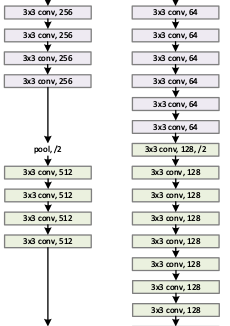
\includegraphics[scale=0.6, trim={0 0 4cm 0},clip]{images/resnet_crop.png}};
				\end{tikzpicture}
				
			}
			\onslide<2->{
				\begin{tikzpicture}
					
					\node[inner sep=0pt] (A) at (5.2,3.8)
					{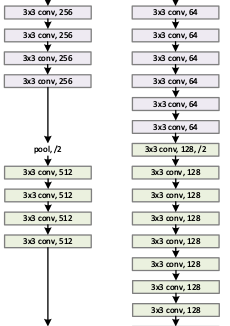
\includegraphics[scale = 0.6]{images/resnet_crop.png}};
					\draw[draw=orange,fill=orange!50,solid,rounded corners,opacity=0.3,line width=0.6mm] (5.1,0.4) rectangle (7.9,1.9);
					\draw[draw=orange,fill=orange!50,solid,rounded corners,opacity=0.3,line width=0.6mm] (5.1,3.8) rectangle (7.9,5.3);
				\end{tikzpicture}
				    
			}  
		\end{overlayarea}
		
		
		
		\column{0.5\textwidth}
		\begin{overlayarea}{\textwidth}{\textheight}
			\begin{itemize}
				\justifying
				\item<1-> Suppose we have been able to train a shallow neural network well
				\item<2-> Now suppose we construct a deeper network which has few more layers (in orange)
				\item<3-> Intuitively, if the shallow network works well then the deep network should also work well by simply learning to compute identity functions in the new layers
				\item<4-> Essentially, the solution space of a shallow neural network is a subset of the solution space of a deep neural network
			\end{itemize}
		\end{overlayarea}
	\end{columns}
\end{frame}

%%%%%%%%%%%%%%%%%%%%%%%%%%%%%%%%%%%%%%%%%%%%%%%%%%%%%%%%%%%%%%%%%%%%%%%%%%%%%%

\begin{frame}
	\begin{columns}
		\column{0.5\textwidth}
		\begin{overlayarea}{\textwidth}{\textheight}
			\vspace{4mm}
			\hspace{6mm}
			\onslide<1->{\begin{figure}
				\begin{center}
					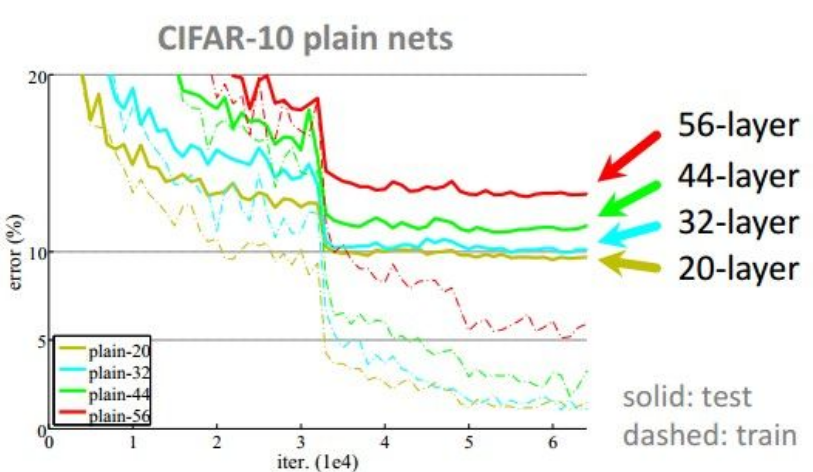
\includegraphics[scale=0.25]{images/plain_nets.png}
				\end{center}
				\end{figure}
				
			}
			
		\end{overlayarea}
		
		\column{0.5\textwidth}
		\begin{overlayarea}{\textwidth}{\textheight}
			\begin{itemize}
				\justifying
				\item<1-> But in practice it is observed that this doesn't happen
				\item<2-> Notice that the deep layers have a higher error rate on the test set
				%\item<3-> 
				%\item<2-> Residual Networks try to fix this issue
				%\item<3-> What if we enable it to learn only a residual function of the input?
			\end{itemize}
		\end{overlayarea}
	\end{columns}
\end{frame}

%%%%%%%%%%%%%%%%%%%%%%%%%%%%%%%%%%%%%%%%%%%%%%%%%%%%%%%%%%%%%%%%%%%%%%%%%%%%%%

\begin{frame}
	\begin{columns}
		\column{0.5\textwidth}
		\begin{overlayarea}{\textwidth}{\textheight}
			\begin{tikzpicture}
				\node (T) at (0,0){};
				\node [rectangle, draw=black, minimum width=2cm, minimum height=4mm, fill=red!50] (A) at ($(T) + (3,0)$) {}; 
				\node [rectangle, draw=black, minimum width=2cm, minimum height=4mm, fill=red!50] (B) at ($(A) + (0,-1)$) {}; 
				\draw [line width=1] [->] (A) -- (B);
				\node (H) at ($(B) + (0,-1)$ ) {$H(x)$};
				\node (x) at ($(A) + (0,1)$ ) {$x$};
				\node (relu1) at ($(A) + (0.4,-0.5)$ ) {\tiny{$relu$}};
				\node (relu2) at ($(B) + (0.4,-0.5)$ ) {\tiny{$relu$}};
				\draw [line width=1] [->] (x) -- (A);
				\draw [line width=1] [->] (B) -- (H);
				\onslide<3->{
					\node [rectangle, draw=black, minimum width=2cm, minimum height=4mm, fill=red!50] (C) at ($(H) + (0,-1.8)$) {}; 
					\node [rectangle, draw=black, minimum width=2cm, minimum height=4mm, fill=red!50] (D) at ($(C) + (0,-1)$) {}; 
					\draw [line width=1] [->] (C) -- (D);
					\node (F1) at ($(D) + (-0.5,-0.5)$ ) {\tiny{$F(x)$}};
					\node (x1) at ($(C) + (0,1)$ ) {$x$};
					\node (relu11) at ($(C) + (0.4,-0.5)$ ) {\tiny{$relu$}};
					\node (relu21) at ($(D) + (0.4,-0.5)$ ) {\tiny{$relu$}};
					\draw [line width=1] [->] (x1) -- (C);
					
					\node [circle,draw,line width=1] (E) at ($(D) + (0,-1)$) {};
					\draw [line width=1] [->] (D) -- (E);
					%\draw ($(x1) + (0,-0.3)$) edge[line width=1,bend right,in=90, out=90,->] ($(H1) + (0,-0.3)$){};
					\draw[->,line width=1, color=blue] ($(x1) + (0,-0.3)$) to [out=0,in=90] ($(relu21) + (1.5,1)$) to [out=-90,in=0] (E) {};
					\node (H1) at ($(E) + (0,-0.5)$ ) {\footnotesize{$H(x)=F(x)+x$}};
					\node [color=blue](I1) at ($(relu21) + (2.2,1)$) {\footnotesize{Identity}};
				}
			\end{tikzpicture}
		\end{overlayarea}
		
		\column{0.5\textwidth}
		\begin{overlayarea}{\textwidth}{\textheight}
			\begin{itemize}
				\item<1-> Consider any two stacked layers in a CNN
				\item<2-> The two layers are essentially learning some function of the input
				\item<3-> What if we enable it to learn only a residual function of the input?
			\end{itemize}
		\end{overlayarea}
	\end{columns}
\end{frame}

%%%%%%%%%%%%%%%%%%%%%%%%%%%%%%%%%%%%%%%%%%%%%%%%%%%%%%%%%%%%%%%%%%%%%%%%%%%%%%

\begin{frame}
	\begin{columns}
		\column{0.5\textwidth}
		\begin{overlayarea}{\textwidth}{\textheight}
			\begin{tikzpicture}
				\node (T) at (0,0){};
				\node [rectangle, draw=black, minimum width=2cm, minimum height=4mm, fill=red!50] (A) at ($(T) + (3,0)$) {}; 
				\node [rectangle, draw=black, minimum width=2cm, minimum height=4mm, fill=red!50] (B) at ($(A) + (0,-1)$) {}; 
				\draw [line width=1] [->] (A) -- (B);
				\node (H) at ($(B) + (0,-1)$ ) {$H(x)$};
				\node (x) at ($(A) + (0,1)$ ) {$x$};
				\node (relu1) at ($(A) + (0.4,-0.5)$ ) {\tiny{$relu$}};
				\node (relu2) at ($(B) + (0.4,-0.5)$ ) {\tiny{$relu$}};
				\draw [line width=1] [->] (x) -- (A);
				\draw [line width=1] [->] (B) -- (H);
				
				\node [rectangle, draw=black, minimum width=2cm, minimum height=4mm, fill=red!50] (C) at ($(H) + (0,-1.8)$) {}; 
				\node [rectangle, draw=black, minimum width=2cm, minimum height=4mm, fill=red!50] (D) at ($(C) + (0,-1)$) {}; 
				\draw [line width=1] [->] (C) -- (D);
				\node (F1) at ($(D) + (-0.5,-0.5)$ ) {\tiny{$F(x)$}};
				\node (x1) at ($(C) + (0,1)$ ) {$x$};
				\node (relu11) at ($(C) + (0.4,-0.5)$ ) {\tiny{$relu$}};
				\node (relu21) at ($(D) + (0.4,-0.5)$ ) {\tiny{$relu$}};
				\draw [line width=1] [->] (x1) -- (C);
				
				\node [circle,draw,line width=1] (E) at ($(D) + (0,-1)$) {};
				\draw [line width=1] [->] (D) -- (E);
				%\draw ($(x1) + (0,-0.3)$) edge[line width=1,bend right,in=90, out=90,->] ($(H1) + (0,-0.3)$){};
				\draw[->,line width=1, color=blue] ($(x1) + (0,-0.3)$) to [out=0,in=90] ($(relu21) + (1.5,1)$) to [out=-90,in=0] (E) {};
				\node (H1) at ($(E) + (0,-0.5)$ ) {\footnotesize{$H(x)=F(x)+x$}};
				\node [color=blue](I1) at ($(relu21) + (2.2,1)$) {\footnotesize{Identity}};
				
			\end{tikzpicture}
		\end{overlayarea}
			
		\column{0.5\textwidth}
		\begin{overlayarea}{\textwidth}{\textheight}
			\begin{itemize}
				\justifying
				\item<1-> Why would this help?
				\item<2-> Remember our argument that a deeper version of a shallow 
				network would do just fine by learning identity transformations in the new layers
				\item<3-> This identity connection from the input allows a ResNet to retain a copy of the input
				\item<4-> Using this idea they were able to train really deep networks
			\end{itemize}
		\end{overlayarea}
	\end{columns}
\end{frame}
		
%%%%%%%%%%%%%%%%%%%%%%%%%%%%%%%%%%%%%%%%%%%%%%%%%%%%%%%%%%%%%%%%%%%%%%%%%%%%%%			
			
\begin{frame}
	\begin{columns}
		\column{0.5\textwidth}
		\begin{overlayarea}{\textwidth}{\textheight}
			\vspace{0.3cm}
			\begin{figure}
				\begin{center}
					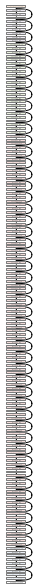
\includegraphics[scale=0.29]{images/resNet_layers.png}
					\caption*{ResNet, \textcolor{red} {152 layers}}
				\end{center}
			\end{figure}
		\end{overlayarea}
		\column{0.5\textwidth}
		\begin{overlayarea}{\textwidth}{\textheight}
			\begin{block}{$1^{st}$ place in all five main tracks}
				\begin{itemize}
					\justifying
					\item<1-> \textbf{ImageNet Classification:}\hspace{-2mm} ``Ultra-deep'' \textcolor{red}{152-layer} nets
					\item<2-> \textbf{ImageNet Detection:} \textcolor{red}{$16$\%} better than the 2nd best system
					\item<3-> \textbf{ImageNet Localization:} \textcolor{red}{$27$\%} better than the 2nd best system
					\item<4-> \textbf{COCO Detection:} \textcolor{red}{$11$\%} better than the 2nd best system
					\item<5-> \textbf{COCO Segmentation:} \textcolor{red}{$12$\%} better than the 2nd best system
				\end{itemize}
			\end{block}
		\end{overlayarea}
	\end{columns}
\end{frame}

%%%%%%%%%%%%%%%%%%%%%%%%%%%%%%%%%%%%%%%%%%%%%%%%%%%%%%%%%%%%%%%%%%%%%%%%%%%%%%

\begin{frame}
	\begin{columns}
		\column{0.5\textwidth}
		\begin{overlayarea}{\textwidth}{\textheight}
			\vspace{0.3cm}
			\begin{figure}
				\begin{center}
					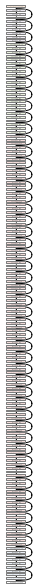
\includegraphics[scale=0.29]{images/resNet_layers.png}
					\caption*{ResNet, \textcolor{red} {152 layers}}
				\end{center}
			\end{figure}
		\end{overlayarea}
		\column{0.5\textwidth}
		\begin{overlayarea}{\textwidth}{\textheight}
			\begin{block}{Bag of tricks}
				\begin{itemize}
					\justifying
					\item<1-> Batch Normalizaton after every CONV layer
					\item<2-> Xavier/2 initialization from [He et al]
					\item<3-> SGD + Momentum(0.9)
					\item<4-> Learning rate:0.1, divided by 10 when validation error plateaus
					\item<5-> Mini-batch size 256
					\item<6-> Weight decay of 1e-5
					\item<7-> No dropout used
				\end{itemize}
			\end{block}
		\end{overlayarea}
	\end{columns}
\end{frame}

